\chapter{集成学习}
\label{chap:ensemble-learning}

信用风险模型可能利用不同的预测信息：线性模型概括全局趋势，决策树表达局部交互；两棵树也可能因训练样本不同而作出不同判断。将这些预测组合起来，有机会减少单个模型遗漏结构或受训练波动影响造成的误差。\term{集成学习}（ensemble learning）研究成员模型的生成与输出组合，并分析成员之间的依赖如何影响新样本预测。

为了说明怎样组合预测，设训练集为
\[
  D_n=\{(\bm{x}_i,y_i)\}_{i=1}^{n},
\]
学习过程产生$M\geq1$个\term{成员模型}$h_1,\ldots,h_M$，每个成员都能对新输入给出一份预测。用$\mathcal{C}_{\bm{x}}$表示在当前输入处把这些预测合为一个输出的组合规则，得到\term{集成模型}
\begin{equation}
  H(\bm{x})
  =\mathcal{C}_{\bm{x}}\bigl(h_1(\bm{x}),\ldots,h_M(\bm{x})\bigr).
  \label{eq:ensemble-combination}
\end{equation}
组合规则可以固定，也可以根据输入调整成员权重；固定时省略下标$\bm{x}$。本章主要讨论监督预测。成员若都预测同一个回归目标，可以采用等权平均
\[
  H(\bm{x})=\frac{1}{M}\sum_{m=1}^{M}h_m(\bm{x}),
\]
也可以用非负权重$w_m$作加权平均，其中$\sum_m w_m=1$。分类成员则可能输出硬标签、类别得分或类别概率。硬标签对应类别投票，同尺度得分或同类概率可逐类平均后决策；混合不同输出前，需要把它们转换为含义一致的量。

组合之前需要明确输出的数值含义。直接平均不同尺度的分类得分，会使数值范围较大的成员占据更大作用；平均类别概率则保持概率向量形式，但它与真实类别频率是否对应仍需检验。回归均值、分位数和分布，以及分类标签、排序和概率各有评价对象，沿用前两章的区分。

组合能否减少预测错误，还取决于成员怎样产生。若各成员在同一区域都遗漏了同一关系，平均或投票仍会保留这一共同错误；若成员的错误发生在不同样本上，组合才有机会修正其中一部分。成员的预测能力与错误之间的依赖需要一起考虑，单纯增加成员数量并不保证风险下降。

围绕成员生成与组合的关系，本章介绍三类方法。Bagging让同一学习算法在不同重采样数据上分别训练，再平均或投票，主要处理训练样本扰动带来的预测波动。Boosting让新成员针对当前组合的不足训练，用一轮轮修正形成最终预测。Stacking则把已有成员的预测作为新输入，另外训练一个负责组合的模型；为避免这个模型学到成员对训练样本的过度拟合，需要使用未参与相应成员拟合的样本预测。三者分别改变训练数据、逐轮学习目标或组合规则，回答的是不同的改进问题。

图\ref{fig:ensemble-three-mechanisms}在同一预测任务中比较这三种训练依赖。给定原训练数据后，Bagging成员可分别训练；Boosting的新成员依赖前轮组合产生的修正信号；Stacking的组合层依赖成员在留出样本上的预测。依赖关系既决定哪些计算可以并行，也决定二阶段训练需要隔离哪些样本信息。

\begin{figure*}[htbp]
  \centering
  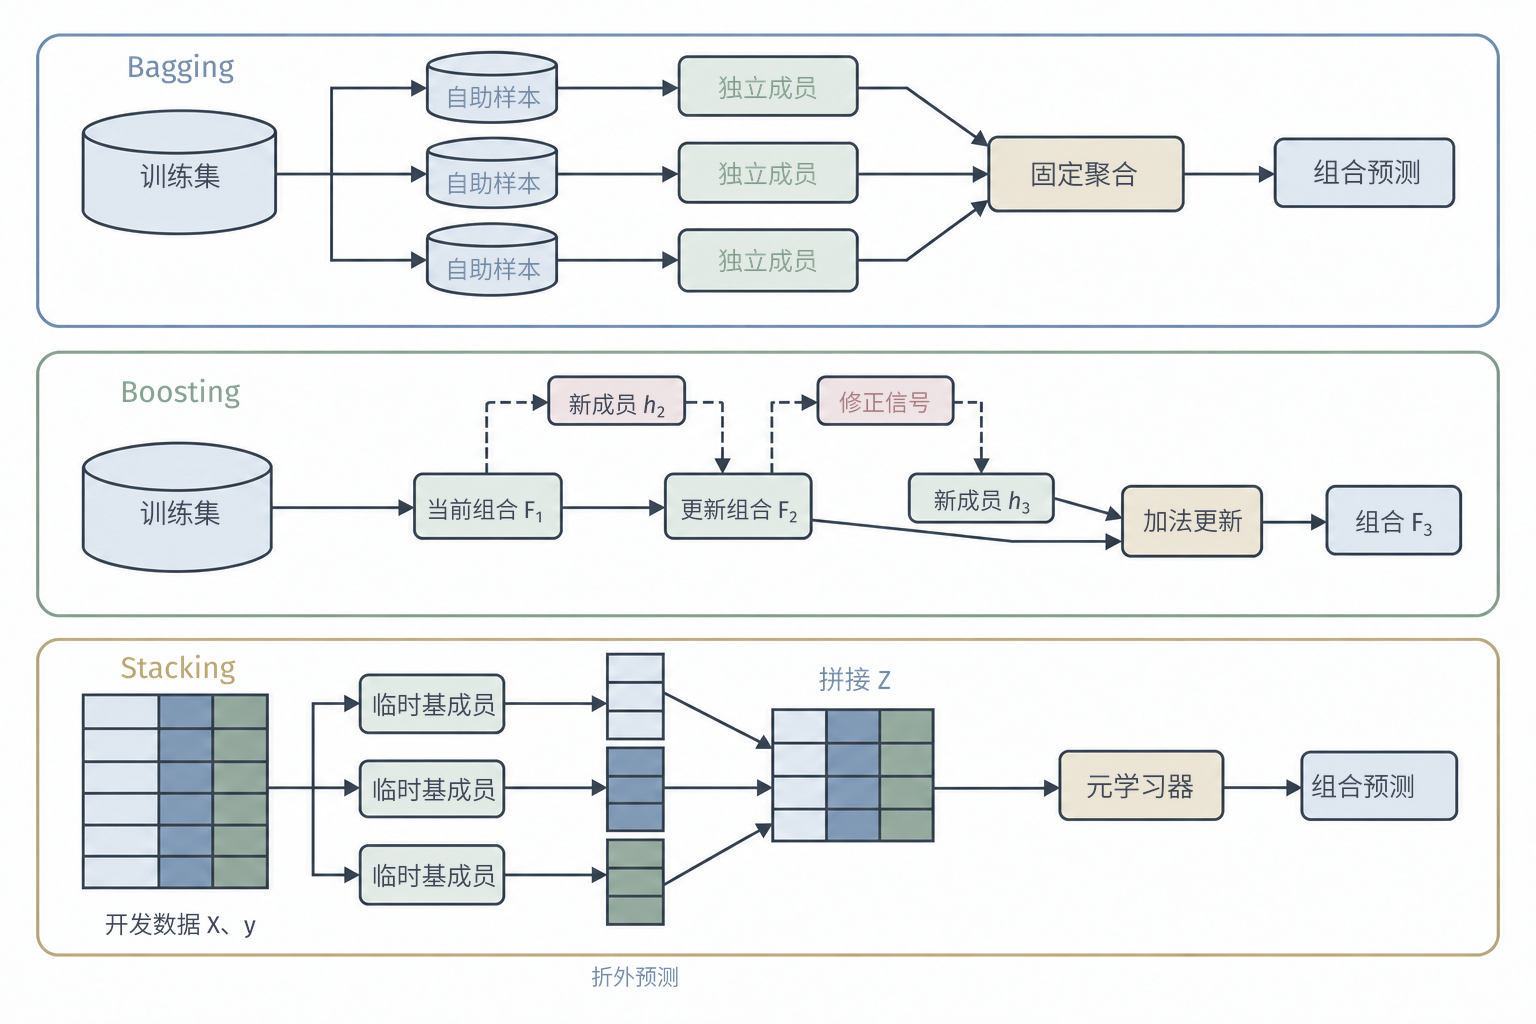
\includegraphics[width=130.048mm]{figures/04-classic-models/00-shared/generated/ensemble-three-mechanisms/figure.png}
  \caption{Bagging、Boosting与Stacking的成员生成及组合关系。实线连接训练与预测步骤，虚线传递当前组合形成的修正信号。三类机制的成员依赖及组合规则不同；示意流程允许采用不同成员模型。}
  \label{fig:ensemble-three-mechanisms}
\end{figure*}


\section{基于Bagging的集成}
\label{sec:ensemble-bagging}

单棵树的预测可能对训练样本很敏感。例如，根节点上两个候选分裂的得分很接近，替换少量训练记录就可能让另一分裂胜出；后续节点收到的样本随之改变，最终预测也可能不同。这正是上一节说的“方差大”。若能从同一总体反复抽取多份独立的训练集，分别建树后平均，各树因样本偶然性产生的波动就会相互抵消。困难在于现实中通常只有一份训练数据，不可能真的回到总体重新采样。

统计学的\emph{自助法}（bootstrap）提供了一个巧妙的替代：既然拿不到总体，就把手头这份样本当作总体的“缩影”，从中\emph{有放回地}重复抽样。具体做法是从$n$条记录里每次随机抽一条、记下后放回，连抽$n$次，得到一份同样大小的“自助样本”。由于是有放回抽取，同一条记录可能被抽中两三次，另一些记录则一次都没被抽中，于是每份自助样本都是原数据的一个略有不同的版本，模拟了“换一批数据”的效果。\term{装袋法}（bootstrap aggregating, Bagging）就是从现有训练集抽取多份自助样本，分别训练成员，再对数值预测取平均或对类别投票。重采样让同一学习算法看到不同的记录组合，聚合则让一次样本扰动不再独自决定最终预测。若所有成员在同一区域都存在相同偏差，平均仍会保留这个偏差；Bagging主要针对的是训练扰动带来的波动，因此最适合本身容易波动（低偏差、高方差）的学习器，如深的决策树\scite{breiman1996bagging}。

\subsection{Bagging}
\label{sec:ensemble-bagging-bootstrap}

\subsubsection{模型结构}

Bagging保留$M$个由同一基学习器训练的成员，预测时按固定规则聚合。回归采用等权平均，分类采用多数投票或同类概率平均；成员之间没有逐轮修正关系，组合层也不再学习一组权重。成员的函数形式由基学习器决定，下面用自助采样使同一算法产生不同的成员。

图\ref{fig:ensemble-error-dependence}说明平均为何需要成员之间存在差异。成员各自的波动可能在平均中抵消；如果所有成员都犯同一种错误，重复增加这样的成员仍会保留共同误差。

\begin{figure*}[htbp]
  \centering
  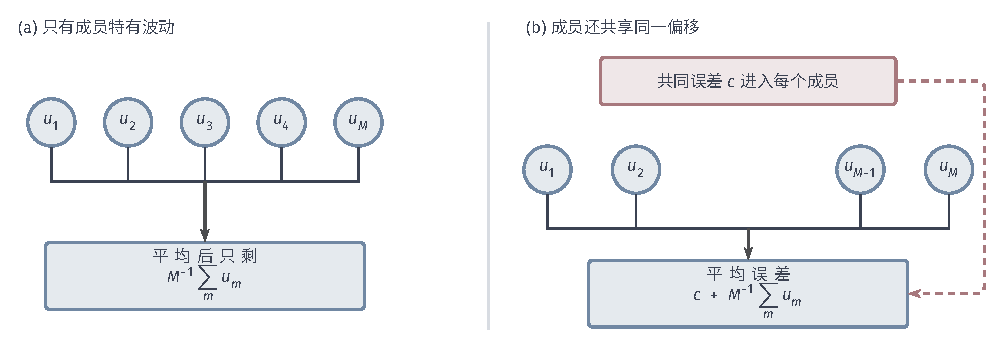
\includegraphics[width=169.000mm]{figures/04-classic-models/00-shared/tikz/ensemble-error-dependence/figure.pdf}
  \caption{成员误差依赖与平均的作用。左图表示只有成员特有波动时，平均可以随成员数增加而削弱这些波动；右图表示所有成员还共享误差$c$时，共同项仍保留在平均预测中。图中成员数量与符号只用于说明机制，不表示实测误差。}
  \label{fig:ensemble-error-dependence}
\end{figure*}

\subsubsection{参数学习}

对第$m$个成员，从$\{1,\ldots,n\}$中独立、等概率、有放回地抽取$n$次索引，所得多重集合记为$I^{(m)}$。有放回抽样使部分记录重复进入成员训练，也使部分记录留在该成员之外。学习算法$\mathcal{A}$在相应自助样本上训练出
\[
  h_m=\mathcal{A}\!\left(D_n^{(m)}\right),
  \qquad
  D_n^{(m)}=\{(\bm{x}_i,y_i):i\in I^{(m)}\}.
\]
回归通常平均$h_m(\bm{x})$；分类可以投票，也可以在成员输出具有同一语义时平均逐类得分或概率。可以改变自助样本大小或采用其他成员算法。此时仍需检验重采样是否使成员在新样本上产生互补预测。

\paragraph{构造袋外预测}

一份大小为$n$的标准自助样本没有抽中原始样本$i$的概率为
\begin{equation}
  \mathbb{P}\!\left(i\notin I^{(m)}\right)
  =
  \left(1-\frac{1}{n}\right)^n
  \longrightarrow e^{-1}.
  \label{eq:ensemble-oob-probability}
\end{equation}
因此，每个成员平均约有$36.8\%$的原始样本未参与其训练。这个副产品非常有用：评估模型通常要另外留出一份验证集，而Bagging免费送来了一份——对某个成员而言，那些它没见过的样本正好可以用来检验它，既不必额外切分数据，也没有浪费训练记录。这些样本构成该成员的\term{袋外样本}（out-of-bag sample, OOB sample）。反过来，对每个训练样本$i$，可以只收集没有使用它训练的成员预测。令
\[
  \mathcal{M}_{i}^{\mathrm{OOB}}
  =\{m:i\notin I^{(m)}\},
\]
当$\mathcal{M}_{i}^{\mathrm{OOB}}$非空时，回归的袋外预测可写为
\begin{equation}
  \widehat{y}_{i}^{\mathrm{OOB}}
  =
  \frac{1}{|\mathcal{M}_{i}^{\mathrm{OOB}}|}
  \sum_{m\in\mathcal{M}_{i}^{\mathrm{OOB}}}h_m(\bm{x}_i),
  \label{eq:ensemble-oob-prediction}
\end{equation}
分类则对同一成员集合投票或平均类别输出。图\ref{fig:ensemble-bagging-oob}按样本收集符合条件的成员：每个样本的袋外预测由其未参与训练的成员子集给出，子集随样本变化。

\begin{figure*}[htbp]
  \centering
  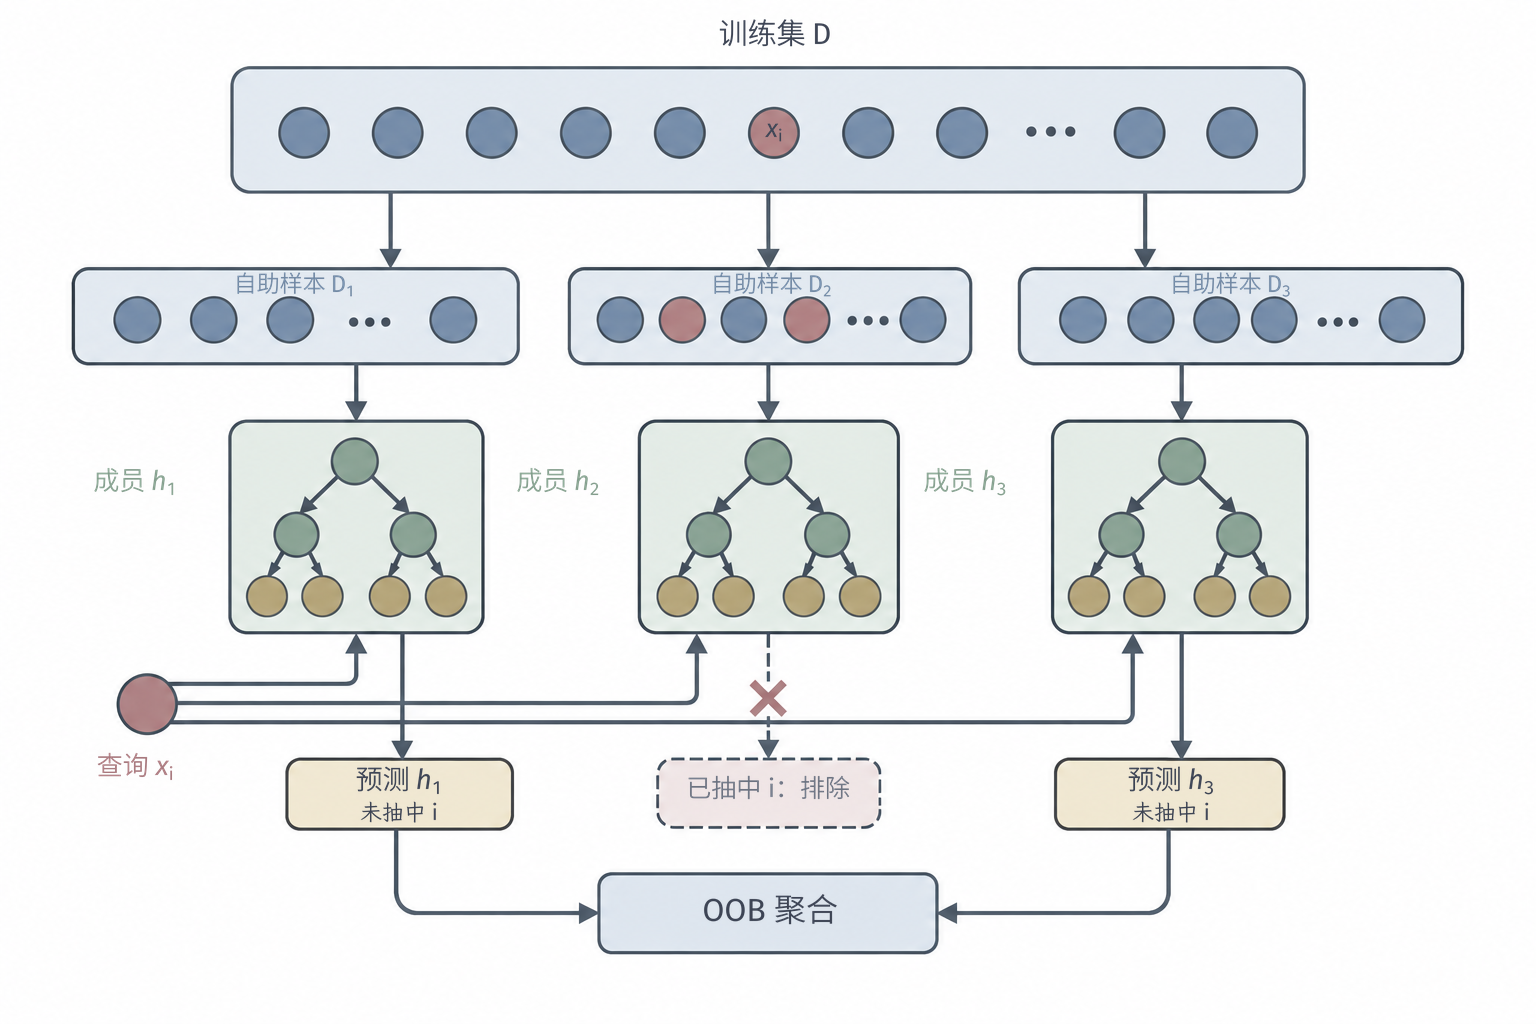
\includegraphics[width=130.048mm]{figures/04-classic-models/00-shared/generated/ensemble-bagging-oob/figure.png}
  \caption{Bagging训练与袋外预测。每个成员只使用其自助样本训练；对训练样本$\bm{x}_i$，袋外预测只聚合未抽中$i$的成员。索引与集合展示样本和成员的对应关系；成员数有限时，各样本得到的袋外预测数量不同。}
  \label{fig:ensemble-bagging-oob}
\end{figure*}

袋外预测使当前标签与产生该预测的成员训练分离，可用于绘制树数—损失曲线、内部误差估计和置换重要性。可用成员数随机变化，自助训练集又相互重叠，这一数据结构与固定折的交叉验证不同。成员数很小时，某些样本可能没有足够的袋外预测。

反复用袋外结果选择结构、树数或特征处理，会使袋外误差成为开发证据；最终冻结流程需要另用测试数据评价。时间序列、分组样本或空间相关数据还要求自助抽样尊重依赖单位；逐行重采样会破坏原有数据结构。袋外结果的解释还依赖抽样单位与未来使用的数据制度。

\paragraph{选择成员规模与训练预算}

给定原数据后，独立的重采样及训练可分配给不同计算单元。评价并行收益时，需要同时计入总工作量与实际经过时间：若单个成员的训练和预测成本分别为$C_{\mathrm{train}}$与$C_{\mathrm{pred}}$，朴素实现的总工作量仍约随$M C_{\mathrm{train}}$和$M C_{\mathrm{pred}}$增长。模型存储也通常随成员数量增加。

在固定训练集上增加独立随机成员，主要减少有限次抽样的Monte Carlo误差；等权平均逐渐逼近该随机训练机制的期望预测。原数据的抽样误差和模型失配仍影响这一期望，共同误差也会留在组合中。实践中可以观察袋外损失随成员数的变化，在曲线趋于稳定后停止增加成员，但这个停止规则也属于模型选择过程。

可以用一个固定输入处的简化误差模型看清这一区别。设第$m$个成员相对真实回归均值的误差为$b+C+U_m$，其中$b$为固定偏差，$C$为所有成员共享的零均值训练数据误差，$U_m$为各自的零均值随机训练误差。假设$C$与各$U_m$不相关，各$U_m$彼此不相关，方差分别为$\tau^2$与$\sigma^2$，则平均预测的均方误差为
\[
 \mathbb E\left(b+C+\frac1M\sum_{m=1}^M U_m\right)^2
 =b^2+\tau^2+\frac{\sigma^2}{M}.
\]
给定训练数据后，各成员的随机数可以独立；重新抽取训练数据时，它们仍会共享$C$，因而预测误差相关。例如$b=0$、$\tau^2=1$、$\sigma^2=3$时，单成员均方误差为4，10个成员平均后为1.3；共同方差1不会随树数消失。这个分解说明平均能消除哪部分波动，不保证任意学习器经Bagging后都降低误差。

单树复杂度控制每份样本上的拟合，树数控制随机预测的平均程度。较深树可以表达更细的分区，也可能对扰动更敏感；叶规模与深度限制则可减少极小叶和噪声标签的影响。叶最小样本量、最大深度、类别权重和自助样本大小仍须与成员数共同选择，尤其在标签噪声、极小叶或类别极不平衡时。

\subsection{随机森林}
\label{sec:ensemble-random-forest}

\subsubsection{模型结构}

树Bagging改变了训练记录，但未必让树的结构有足够差异。例如，房屋面积若在多数自助样本中都是最强的分裂特征，各树就会几乎都先按面积划分，继而在相似区域作出相似错误。回到章首的投票算例：成员越相关，投票收益越小；这些树虽然看到的样本不同，却因为同一个强特征而“想法雷同”，高度相关。增加树数能稳定平均，却不能自动消除成员共同的错误。

\term{随机森林}（random forest）的对策是故意“限制每棵树的视野”：在自助采样之外加入节点级特征随机化，每个节点先随机抽取一组候选特征，只在这组中搜索分裂。面积不在当前候选组时，树就被迫尝试房龄或其他特征，由此长出不同的划分。乍看这让单棵树变差了（它有时用不上最强的特征），但换来的是树与树之间相关性降低，使平均真正发挥作用；这是一个“牺牲单个成员准确度、换取成员多样性”的典型权衡。树仍按第\ref{sec:regression-trees}节或第\ref{sec:classification-trees}节的任务准则形成叶输出；随机化改变的是本次分裂可使用的信息，用来减弱各树对少数强特征的共同依赖\scite{breiman2001randomforests}。

\subsubsection{参数学习}

训练每棵树时，先抽取自助样本，再递归生长各节点：随机选取候选特征，在这些特征上按任务损失搜索分裂，直到达到停止条件，最后计算各叶的预测值。不同树使用各自的抽样与特征随机数，可以分别训练。

节点候选特征数同时影响单树可用的信息和不同树的分裂差异。候选数接近全部特征时，森林更接近普通的树Bagging；候选数较小时，不同树更可能采用不同分裂，但单棵树也更容易错过当前节点上的有效特征。合适的候选规模取决于特征冗余、样本量和树深，可在固定验证协议下比较。

\subsection{极度随机树（Extra Trees）}
\label{sec:ensemble-extra-trees}

\subsubsection{模型结构}

随机森林虽然随机选择候选特征，阈值仍通过当前节点的数据搜索。如果同一个数值特征有很多候选切分点，每棵树仍要承担相应搜索成本，而且不同树可能继续选中接近的最佳阈值。\term{极度随机树}（extremely randomized trees, Extra Trees）进一步随机生成候选切分点，再从这些随机候选中选取得分较好的分裂。它同时减少阈值搜索并增加树之间的差异，代价是单棵树放弃了在全部阈值中寻找最佳分裂。原始方法通常让各树使用完整训练集，把差异主要交给特征与阈值随机化；具体软件也可能允许额外使用自助采样\scite{geurts2006extra}。

\subsubsection{参数学习}

在每个节点，先抽取候选特征，为这些特征生成随机阈值，再按分类不纯度或回归损失比较候选分裂；选定分裂后继续递归，叶输出仍按所属任务估计。阈值的随机生成替代了遍历全部候选值的步骤，训练其他部分沿用树模型。

随机阈值减少了穷举候选切分的工作，也会让单棵树偏离当前样本上的最佳贪心分裂。组合是否改善，取决于单树预测能力下降与成员依赖减弱之间的平衡。候选特征数、每个特征的随机阈值数、叶最小样本量以及是否采用自助采样共同决定这个平衡；增加随机化能否降低测试损失，需要在同一数据与预算下检验。

\subsection{模型对比与总结}
\label{sec:ensemble-bagging-comparison}

图\ref{fig:ensemble-tree-randomization}沿一棵树的构造路径比较三种随机化位置。树Bagging主要改变成员看到的训练样本；随机森林还在每个节点抽取候选特征；Extra Trees继续把随机性放入候选阈值。三者继续以任务准则比较分裂，差别在于进入贪心搜索的样本、特征和阈值。

\begin{figure*}[htbp]
  \centering
  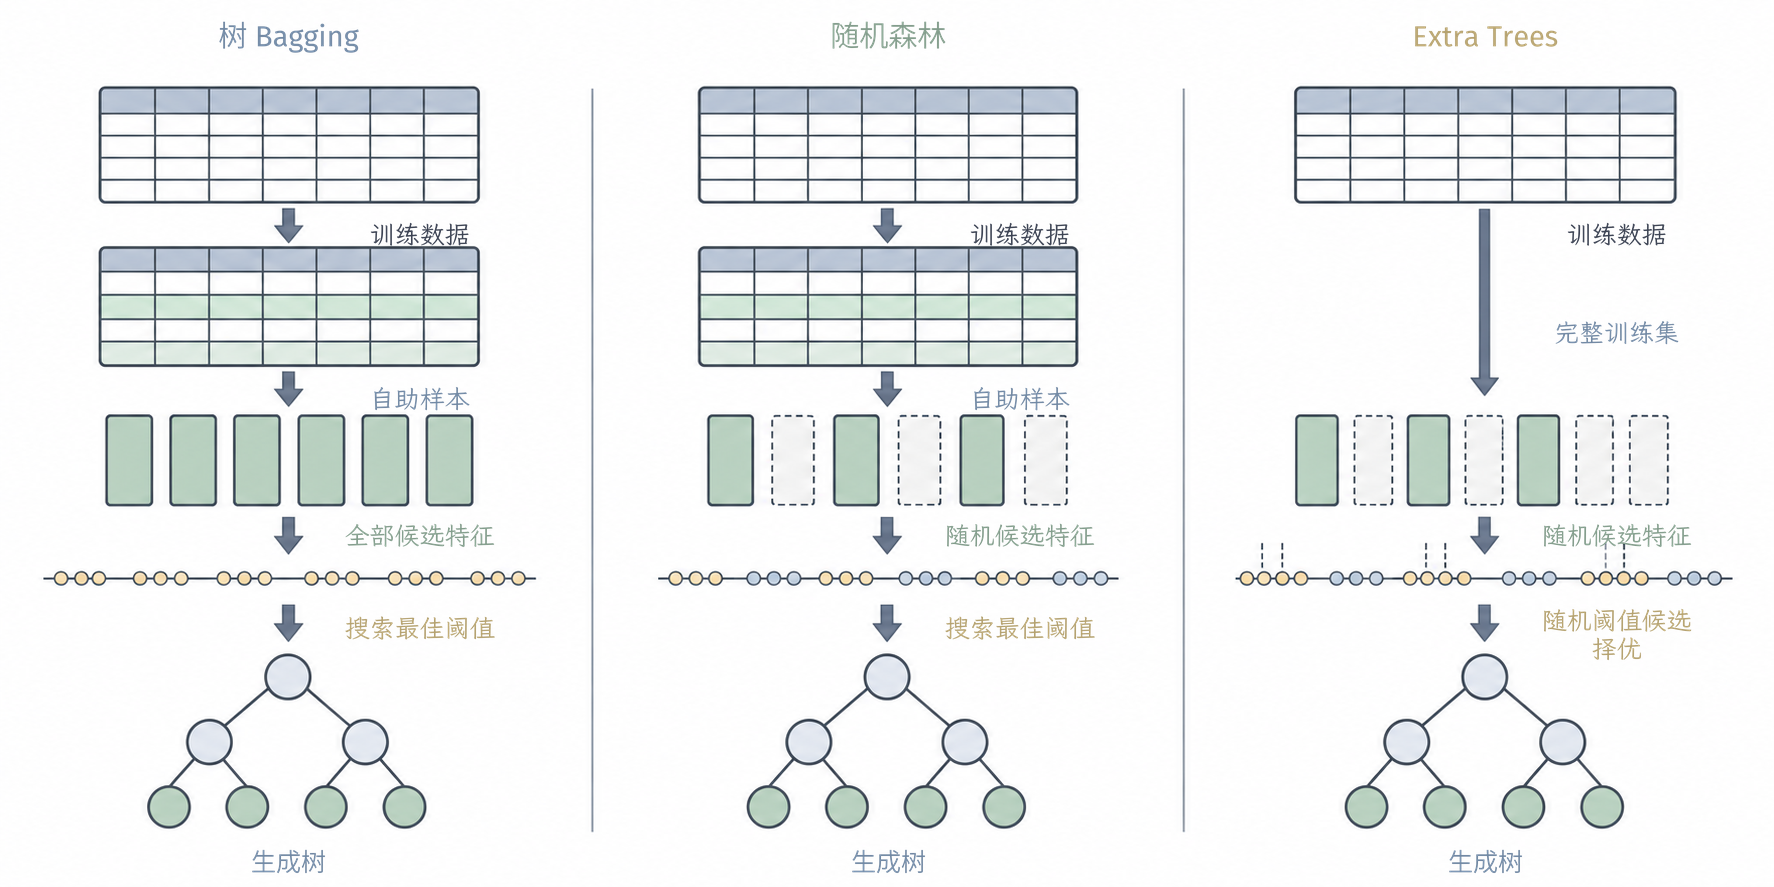
\includegraphics[width=150.199mm]{figures/04-classic-models/00-shared/generated/ensemble-tree-randomization/figure.png}
  \caption{树Bagging、随机森林与Extra Trees的随机化位置。每栏从样本来源出发，依次展示候选特征、候选阈值与成员树；候选选择中的随机性和任务准则约束分别标在相应步骤。每栏首框直接标出训练样本来源：前两栏采用自助采样，Extra Trees栏采用原始方法的完整训练集设定；具体实现也可能额外启用自助采样。}
  \label{fig:ensemble-tree-randomization}
\end{figure*}

三种方法的预测都由树叶输出聚合得到。它们依次改变样本、节点候选特征和候选阈值，训练时仍用任务准则决定分裂与叶值。增加随机化可能减弱共同错误，也可能削弱单树，因此应在相同预算下比较组合预测；表\ref{tab:ensemble-bagging-comparison}列出具体差别。

\begin{table*}[htbp]
  \centering
  \small
  \begin{tabularx}{\linewidth}{@{}>{\raggedright\arraybackslash}p{24mm}*{6}{>{\raggedright\arraybackslash}X}@{}}
    \toprule
    方法 & 样本扰动 & 节点候选特征 & 阈值选择 & 袋外预测 & 成员训练 & 主要边界 \\
    \midrule
    树Bagging & 通常自助采样 & 全部特征 & 在候选中搜索 & 标准自助设定下可用 & 成员间可并行 & 强特征可能使树高度相关 \\
    随机森林 & 通常自助采样 & 随机特征子集 & 在子集内搜索 & 标准自助设定下可用 & 成员间可并行 & 候选数过小会削弱单树 \\
    Extra Trees & 原始方法使用完整训练集；实现可选自助采样 & 随机特征子集 & 生成随机阈值后择优 & 仅在采用自助采样时可用 & 成员间可并行 & 过强随机化会增大单树误差 \\
    \bottomrule
  \end{tabularx}
  \caption{以树为成员时，Bagging、随机森林与Extra Trees的机制比较。表中列出基本构造；比较具体实现时，还需记录抽样设置，并固定树复杂度、成员数和计算预算。}
  \label{tab:ensemble-bagging-comparison}
\end{table*}

原始Extra Trees使用完整训练集，没有标准自助采样形成的袋外预测；若额外启用自助采样，才可按相应未抽中成员构造袋外结果。

Bagging先产生训练差异，再聚合预测以削弱部分波动。固定聚合保留成员共享的遗漏；若希望让新成员针对这些不足训练，就需要根据当前组合产生修正信号。下一节据此转向序贯提升。

\section{基于Boosting的集成}
\label{sec:ensemble-boosting}

Bagging让多个成员分别完成同一个预测任务，再聚合它们的结果。如果这些成员反复在同一批样本上预测偏低，仅增加类似成员并平均，偏低的误差仍会保留。我们可以换一种训练方式：先计算已有组合还错在哪里，再让新成员专门学习一个修正量。

\term{Boosting}（提升）由此构造序贯加法模型：第$t$轮根据已有函数$F_{t-1}$选择新成员及其贡献，以降低指定训练目标。新成员承担的是对已有预测的补充，可以比一个独立完成任务的模型更简单。AdaBoost、梯度提升及现代提升树共享这种逐轮依赖，但它们从错误中提取修正信号的方式不同。

\subsection{前向逐步加法模型}
\label{sec:ensemble-stagewise-additive}

\subsubsection{模型结构}

设$F_0$为初始预测，Boosting经过$T$轮得到
\begin{equation}
  F_T(\bm{x})
  =
  F_0(\bm{x})
  +
  \sum_{t=1}^{T}\alpha_t h_t(\bm{x}),
  \label{eq:ensemble-additive-model}
\end{equation}
其中$h_t$是第$t$个成员，$\alpha_t$控制其贡献。

\subsubsection{参数学习}

为使复杂度惩罚对应真正加入模型的函数，把本轮增量记为$f_t=\alpha_t h_t$。给定损失$\ell$，理想化的第$t$轮直接优化增量：
\begin{equation}
  f_t
  \in
  \argmin_{f\in\mathcal{F}}
  \sum_{i=1}^{n}
  \ell\!\left(
    y_i,
    F_{t-1}(\bm{x}_i)+f(\bm{x}_i)
  \right)
  +\Omega_t(f).
  \label{eq:ensemble-forward-stagewise}
\end{equation}
这里$\mathcal{F}=\{\alpha h:\alpha\in\mathbb{R},h\in\mathcal{H}\}$是由成员函数族$\mathcal{H}$生成的增量函数族，$\Omega_t$是相应复杂度惩罚，也可以取零。

树的叶数惩罚控制分区规模，叶输出范数惩罚控制本轮增量。范数应作用于$f$，使惩罚随实际加入组合的幅度变化；若仅惩罚$h$，它与$\alpha$的相互缩放会改变惩罚却保持预测。

逐步优化固定已有成员，减少了联合搜索变量，但最优范围仅限本轮增量。后文用梯度拟合、二阶目标和收缩构造近似更新。

不同方法将当前预测转换为不同的训练信号。AdaBoost改变训练样本的权重，使当前错分记录在下一轮具有更大影响；梯度提升把损失对当前预测的负梯度作为伪响应；二阶提升树还利用局部曲率近似叶权重和分裂收益。平方损失的负梯度恰为普通响应残差，其他损失则给出不同修正量。损失决定了下一轮成员拟合的对象。

\subsection{AdaBoost}
\label{sec:ensemble-adaboost}

\subsubsection{模型结构}

先考虑二分类。如果每轮都用相同权重训练一个简单分类器，容易分类的多数样本可能反复决定边界，而少量错分样本始终得不到修正。\term{AdaBoost}（adaptive boosting）让错分记录在下一轮占更大权重，使新分类器更多地处理这些记录；同时根据本轮分类器的加权错误率确定它在组合中的贡献。这样，训练下一成员所面对的数据权重会随前面成员的预测改变。

模型以二分类函数作为成员，用加权得分$F_T(\bm{x})=\sum_{t=1}^T\alpha_t h_t(\bm{x})$表示组合，按其正负输出类别。每个成员只给出一个类别判断，投票权重决定该判断在组合中的作用。

\subsubsection{参数学习}

取标签$y_i\in\{-1,1\}$和成员$h_t(\bm{x})\in\{-1,1\}$。初始样本权重为$w_i^{(1)}=1/n$，第$t$轮成员的加权错误率为
\begin{equation}
  \epsilon_t
  =
  \sum_{i=1}^{n}
  w_i^{(t)}
  \mathbb{I}\!\left\{y_i\neq h_t(\bm{x}_i)\right\}.
  \label{eq:ensemble-adaboost-error}
\end{equation}
当$0<\epsilon_t<1/2$时，成员投票权重取
\begin{equation}
  \alpha_t
  =
  \frac{1}{2}
  \log\frac{1-\epsilon_t}{\epsilon_t},
  \qquad
  w_i^{(t+1)}
  =
  \frac{
    w_i^{(t)}
    \exp\!\left[-\alpha_t y_i h_t(\bm{x}_i)\right]
  }{Z_t},
  \label{eq:ensemble-adaboost-update}
\end{equation}
其中$Z_t$使新权重和为1。错分样本满足$y_i h_t(\bm{x}_i)=-1$，权重乘上$e^{\alpha_t}$；正确样本的权重乘上$e^{-\alpha_t}$。

若$\epsilon_t=0$，在这些正权重下当前成员已分对全部训练样本，便直接输出$h_t$并停止，避免将发散系数代入更新（参考\BookSectionRef{sec:boosting}{卷3《基础、理论与可信性》第5章“二分类学习的可学习性”第5.6节“集成学习”}）。其余情况下，最终分类器在预先固定平局规则后按$\operatorname{sign}(\sum_t\alpha_t h_t(\bm{x}))$决策。正的成员贡献要求当前加权错误率小于$1/2$；条件未满足时，可停止本轮、调整训练或采用相应变体。

图\ref{fig:ensemble-adaboost-weight-update}将分类错误与下一轮权重连接起来。当前分类结果先改变样本权重，再由归一化后的权重决定下一轮成员看到的训练分布；错分记录因而获得更大的后续影响。

\begin{figure*}[htbp]
  \centering
  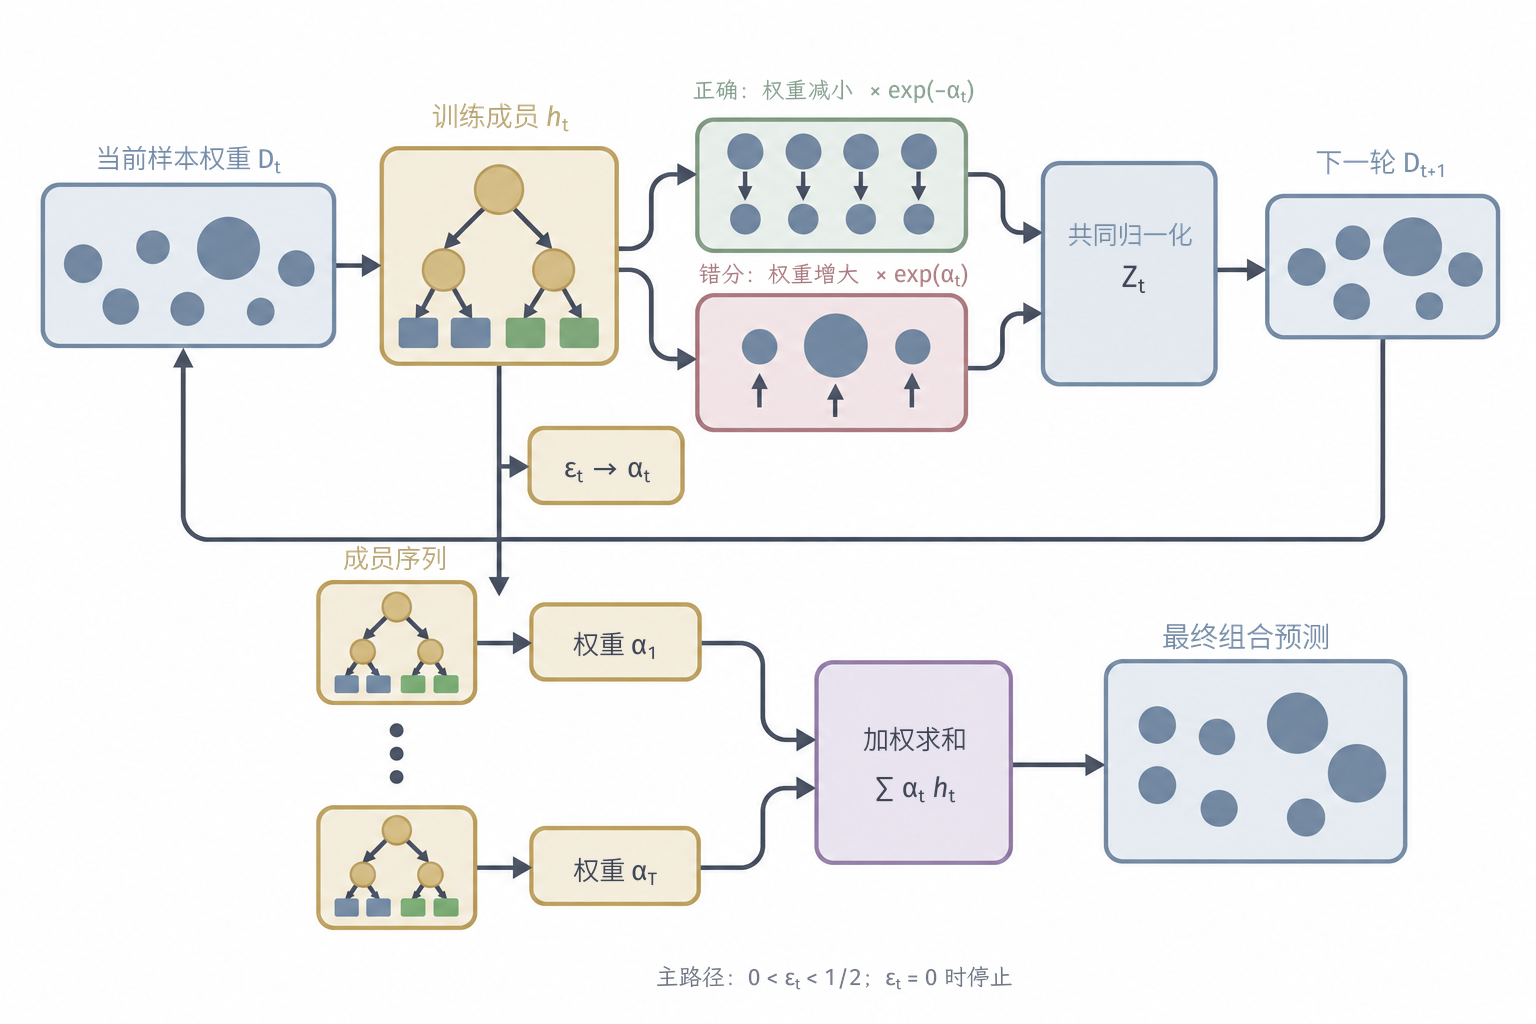
\includegraphics[width=130.048mm]{figures/04-classic-models/00-shared/generated/ensemble-adaboost-weight-update/figure.png}
  \caption{AdaBoost的样本权重更新。分类结果把样本分成正确与错分两路，两路缩放后的权重汇合并归一化，形成下一轮训练分布。实线连接各更新步骤；绿色框标示正确分类样本的减权，红色框标示错分样本的增权。}
  \label{fig:ensemble-adaboost-weight-update}
\end{figure*}

这一更新也可以从指数损失解释。令$F(\bm{x})=\sum_t\alpha_t h_t(\bm{x})$，经验目标为
\[
  \sum_{i=1}^{n}\exp\!\left[-y_iF(\bm{x}_i)\right].
\]
固定$F_{t-1}$后选择$h_t$与$\alpha_t$，在$0<\epsilon_t<1/2$时可以导出式\eqref{eq:ensemble-adaboost-update}。样本重加权由指数损失的逐步优化导出，因此其作用可以通过该目标分析\scite{freund1997boosting,friedman2000adaboost}。

\subsubsection{支持多分类预测场景}

二分类AdaBoost把每个成员的输出编码为$-1$或$+1$，最后用加权得分的正负判类。类别超过两个时，这个标量符号已经不能表示类别竞争。多分类变体需要让成员输出类别或逐类得分，再通过相应的加权投票或得分组合决定类别；样本重加权也要与所选多类损失一致。二分类中要求成员错误率低于$1/2$的条件及其系数公式不能直接沿用，必须按新的类别竞争方式重新推导。

\subsubsection{支持类别概率预测场景}

投票符号只回答类别，许多任务还需要输出事件发生的概率。LogitBoost从加法Logistic回归出发，用二项对数损失确定逐轮更新，再将累积得分转换为概率。它与AdaBoost都逐步加入成员，但修正量来自不同损失；转换后的概率是否准确，仍需根据样本外概率损失和校准情况判断\scite{friedman2000adaboost}。下一节给出一般损失如何导出修正信号的统一构造。

\subsection{梯度提升机与GBDT}
\label{sec:ensemble-gradient-boosting}

\subsubsection{模型结构}

AdaBoost用分类错误调整样本权重，但回归还需要描述“错了多少、向哪边修正”。例如，一个响应为100的样本当前预测为80，平方损失下需要向上修正；另一个响应同为100、当前预测为120的样本则需要向下修正。仅给两条记录增加相同权重，没有直接告诉新成员这两个相反方向。

对于关于预测可微的损失，负梯度给出了每个训练预测降低损失的方向。\term{梯度提升机}（gradient boosting machine, GBM）用基学习器拟合这些负梯度，再把学得的修正加入已有预测。取平方损失$\ell(y,F)=(y-F)^2/2$时，负梯度就是残差$y-F$，其他损失则产生各自的修正信号；序贯加法因而可以用于更一般的任务\scite{friedman2001gradientboost}。

GBM沿用式\eqref{eq:ensemble-additive-model}的加法结构，成员输出连续修正量。成员取回归树时，就是\term{梯度提升决策树}（gradient boosting decision tree, GBDT）；每片叶输出一个常数修正，全部树的修正叠加形成最终得分或数值预测。

\subsubsection{参数学习}

通常从使训练损失最小的常数预测开始：
\begin{equation}
  F_0(\bm{x})=c_0,
  \qquad
  c_0\in\argmin_c\sum_{i=1}^{n}\ell(y_i,c).
  \label{eq:ensemble-gbm-initialization}
\end{equation}
平方损失下$c_0$是响应均值。这里要求存在有限的最小化点；若某种损失与数据组合使最优常数趋于无穷，就需约束预测范围或另定有限初始化。

在第$t$轮，对每个训练样本计算\term{伪残差}（pseudo-residual），即损失在当前预测处的负导数：
\begin{equation}
  r_i^{(t)}
  =
  -
  \left.
  \frac{\partial \ell(y_i,z)}{\partial z}
  \right|_{z=F_{t-1}(\bm{x}_i)}.
  \label{eq:ensemble-pseudo-residual}
\end{equation}
随后用平方误差把这些修正量拟合到成员函数族：
\begin{equation}
  h_t\in\argmin_{h\in\mathcal{H}}
  \sum_{i=1}^{n}\bigl(r_i^{(t)}-h(\bm{x}_i)\bigr)^2.
  \label{eq:ensemble-gbm-gradient-fit}
\end{equation}
此处平方误差衡量成员对负梯度的逼近，即使原任务采用其他损失也使用这一拟合对象。贪心树生长通常给出子问题的近似解。

固定$h_t$后，可以按原损失做整体线搜索，在最小值存在时取
\begin{equation}
  \alpha_t\in\argmin_\alpha
  \sum_{i=1}^{n}
  \ell\!\left(y_i,F_{t-1}(\bm{x}_i)+\alpha h_t(\bm{x}_i)\right).
  \label{eq:ensemble-gbm-line-search}
\end{equation}
此处$\alpha_t$是整棵树或整个成员共享的一个标量。加入预先选择的收缩系数$\eta\in(0,1]$后，
\begin{equation}
  F_t(\bm{x})
  =
  F_{t-1}(\bm{x})
  +
  \eta\alpha_t h_t(\bm{x}).
  \label{eq:ensemble-gradient-boosting-update}
\end{equation}


当$\ell(y,z)=\tfrac12(y-z)^2$时，式\eqref{eq:ensemble-pseudo-residual}给出$y_i-F_{t-1}(\bm{x}_i)$，恰好是普通残差。图\ref{fig:ensemble-boosting-residuals}展示一次这样的更新：新成员拟合的是第二幅图中的残差，再把它的输出加回已有预测。左侧原本偏高的预测随负残差降低，右侧原本偏低的预测随正残差升高；这组数据的平均平方损失也随之下降。

\begin{figure*}[tbp]
  \centering
  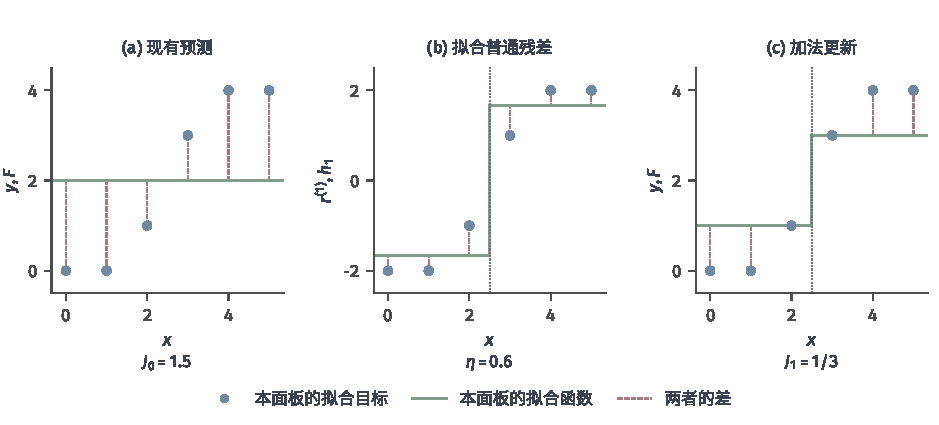
\includegraphics[width=159.000mm]{figures/04-classic-models/00-shared/matplotlib/ensemble-boosting-residuals/figure.pdf}
  \caption{平方损失下的一次梯度提升更新。六个输入为$x=0,\ldots,5$，响应依次为$0,0,1,3,4,4$，常数初始化$F_0=2$。在相邻输入中点中搜索，最小二乘残差树选取阈值$2.5$，两叶输出分别为$-5/3$与$5/3$。取$\eta=0.6$，$F_1=F_0+\eta h_1$在两侧分别为$1$与$3$；平均损失$J_t=(2n)^{-1}\sum_i[y_i-F_t(x_i)]^2$由$1.5$降至$1/3$。蓝点依次表示观测、残差、观测，绿线为各面板的拟合函数，红色虚线为两者之差。数据与更新均为可复核的教学构造，这个普通残差计算依赖平方损失。}
  \label{fig:ensemble-boosting-residuals}
\end{figure*}

分类时则要先明确得分与概率的关系。例如二分类采用$y_i\in\{0,1\}$，令$F$表示对数几率（logit），相应概率与二项对数损失为
\[
  p=\sigma(F)=\frac{1}{1+e^{-F}},\qquad
  \ell(y,F)=\log(1+e^F)-yF.
\]
由于$\partial\ell/\partial F=\sigma(F)-y$，第$t$轮的伪残差为
\[
  r_i^{(t)}=y_i-p_i^{(t-1)},\qquad
  p_i^{(t-1)}=\sigma\!\left(F_{t-1}(\bm{x}_i)\right).
\]


例如$y_i=1$而当前概率为$0.3$时，伪残差为$0.7$，表示损失对得分的修正信号。成员拟合后将增量加到$F$，再经Sigmoid换算概率；修正量与概率因此处于不同数值空间。

对于GBDT，除了整体线搜索，还可以保留平方拟合得到的叶区域$\bm{R}_1^{(t)},\ldots,\bm{R}_{L_t}^{(t)}$，再按原损失分别求每片叶的增量。当各叶内存在有限最小化点时，
\begin{equation}
  \begin{aligned}
    v_j^{(t)}
      &\in\argmin_v
        \sum_{i:\,\bm{x}_i\in\bm{R}_j^{(t)}}
        \ell\!\left(y_i,F_{t-1}(\bm{x}_i)+v\right),\\
    F_t(\bm{x})
      &=F_{t-1}(\bm{x})
        +\eta\sum_{j=1}^{L_t}
        v_j^{(t)}\mathbb{I}\{\bm{x}\in\bm{R}_j^{(t)}\}.
  \end{aligned}
  \label{eq:ensemble-gbm-leaf-update}
\end{equation}
$L_t$表示叶数，各叶分别选择$v_j^{(t)}$并替换原树输出；这与整棵树共用一个$\alpha_t$是两种更新方案。有限叶内最小值不存在时，需要限制输出或增加正则后再更新。回归树在这里承担连续修正量的拟合，最终任务也可以是分类。

\subsubsection{优化泛化能力}

\paragraph{控制逐轮更新幅度与模型复杂度}
学习率、轮数与单树复杂度共同决定加法函数。较小学习率缩小每轮变化，通常需要更多轮才能达到相近训练目标；较深的树可以在单轮表达更高阶交互，也会扩大每轮容量。行采样和列采样进一步引入随机性，早停则依据独立验证轨迹选择轮数。选择学习率时需同时调整轮数，并在给定树复杂度、采样和早停协议下比较。

\paragraph{减弱逐轮拟合对训练样本的依赖}
每轮都使用全部训练样本时，提升树可能反复追踪其中的偶然起伏。随机梯度提升在每轮只用一个随机子样本拟合新成员，使不同轮次面对的记录有所变化。它保留负梯度修正的目标，同时减少本轮参与拟合的样本数。子样本比例过低也可能使修正方向更不稳定，因此采样比例需要与学习率、轮数及树复杂度共同选择\scite{friedman2002stochastic}。

\paragraph{减弱新增成员对既有树的依赖}
提升的后期成员面对的是已有组合留下的残差，可能只修正少量记录，越来越依赖前面树的具体输出。DART在本轮计算修正信号时暂时移除一部分已有树，让新树补充这个不完整组合的预测。加入新树后，算法还会调整新树和被移除树的贡献，再将它们放回组合，避免补回同一缺口时使更新幅度过大。这里扰动的是已有预测，随机梯度提升扰动的则是本轮样本；两者可分别改变新成员依赖的信息，收益仍取决于扰动强度和任务\scite{rashmi2015dart}。

\subsubsection{支持分位数预测场景}

平方损失关注条件均值；若希望按允许的缺货概率确定库存阈值，或预测收入分布中的较低分位点，就需要条件分位数。把第\ref{sec:regression-quantiles}节的分位数损失$\ell(y,z)=\rho_\tau(y-z)$用于提升，成员便学习怎样减少这个分位数目标的偏差。由于损失在$z=y$处不可微，修正信号改用负次梯度，例如约定
\begin{equation}
  r_i^{(t)}
  =\tau-\mathbb{I}\{y_i<F_{t-1}(\bm{x}_i)\},
  \qquad 0<\tau<1.
  \label{eq:ensemble-quantile-pseudo-residual}
\end{equation}
等号处的负次梯度可取$[\tau-1,\tau]$内任意值，这里选端点$\tau$。常数初始化取样本$\tau$分位数，仍用平方误差拟合上述修正量；逐叶更新则最小化原分位数损失，故$v_j^{(t)}$取该叶内普通残差$y_i-F_{t-1}(\bm{x}_i)$的$\tau$分位数，而不是伪残差的均值。

\subsection{XGBoost}
\label{sec:ensemble-xgboost}

\subsubsection{模型结构}

前面介绍的梯度提升用负梯度决定修正方向。用树拟合时，还要选择怎样划分叶区域，以及每个叶应当输出多大的修正。只看当前梯度，没有直接利用损失随修正幅度弯曲的程度；若不断增加叶节点来追逐小幅训练收益，树也可能把样本噪声保留下来。

\term{XGBoost}把叶数和叶权重惩罚写入加法树目标，再用损失的二阶局部近似为叶输出和候选分裂评分。梯度描述向哪边修正，曲率参与决定修正幅度，正则项则限制这次修正使用多复杂的树。大规模训练还要处理稀疏特征、候选阈值与内存访问，原论文围绕这些计算设计了相应系统\scite{chen2016xgboost}。

\subsubsection{参数学习}

设第$t$棵树为$f_t$，损失在当前预测$F_{t-1}(\bm{x}_i)$处的一阶导与二阶导分别为$g_i^{(t)}$和$s_i^{(t)}$。去掉与$f_t$无关的常数后，本轮目标近似为
\begin{equation}
  \widetilde{\mathcal{L}}^{(t)}
  =
  \sum_{i=1}^{n}
  \left[
    g_i^{(t)}f_t(\bm{x}_i)
    +\frac{1}{2}s_i^{(t)}f_t^2(\bm{x}_i)
  \right]
  +\gamma L
  +\frac{\lambda}{2}\sum_{j=1}^{L}v_j^2,
  \label{eq:ensemble-xgboost-objective}
\end{equation}
其中$L$是叶数，$v_j$是第$j$片叶的输出，$\gamma$惩罚新增叶，$\lambda$约束叶权重。若$I_j$表示落入第$j$片叶的样本索引，记
\[
  G_j=\sum_{i\in I_j}g_i^{(t)},
  \qquad
  S_j=\sum_{i\in I_j}s_i^{(t)}.
\]
在$S_j+\lambda>0$时，固定树结构的最优叶权重为
\begin{equation}
  v_j^\star=-\frac{G_j}{S_j+\lambda}.
  \label{eq:ensemble-xgboost-leaf-weight}
\end{equation}
把一个父叶分成左右子叶时，相应近似目标下降量为
\begin{equation}
  \operatorname{Gain}
  =
  \frac{1}{2}
  \left[
    \frac{G_{\mathrm{L}}^2}{S_{\mathrm{L}}+\lambda}
    +
    \frac{G_{\mathrm{R}}^2}{S_{\mathrm{R}}+\lambda}
    -
    \frac{(G_{\mathrm{L}}+G_{\mathrm{R}})^2}
         {S_{\mathrm{L}}+S_{\mathrm{R}}+\lambda}
  \right]
  -\gamma.
  \label{eq:ensemble-xgboost-split-gain}
\end{equation}
式\eqref{eq:ensemble-xgboost-split-gain}把当前损失的梯度、曲率与树复杂度放在同一个分裂准则中。增益评价局部二阶目标在当前分裂下的变化；贪心生长只搜索逐步形成的结构。

图\ref{fig:ensemble-gradient-xgboost}把一阶梯度提升与XGBoost的二阶树评分放在同一计算链中。左图用负梯度定义拟合对象，右图从候选区域的梯度统计计算叶权重和分裂增益；二阶统计扩展了本轮目标的近似信息，但没有改变逐轮加法更新的外层结构。

\begin{figure*}[htbp]
  \centering
  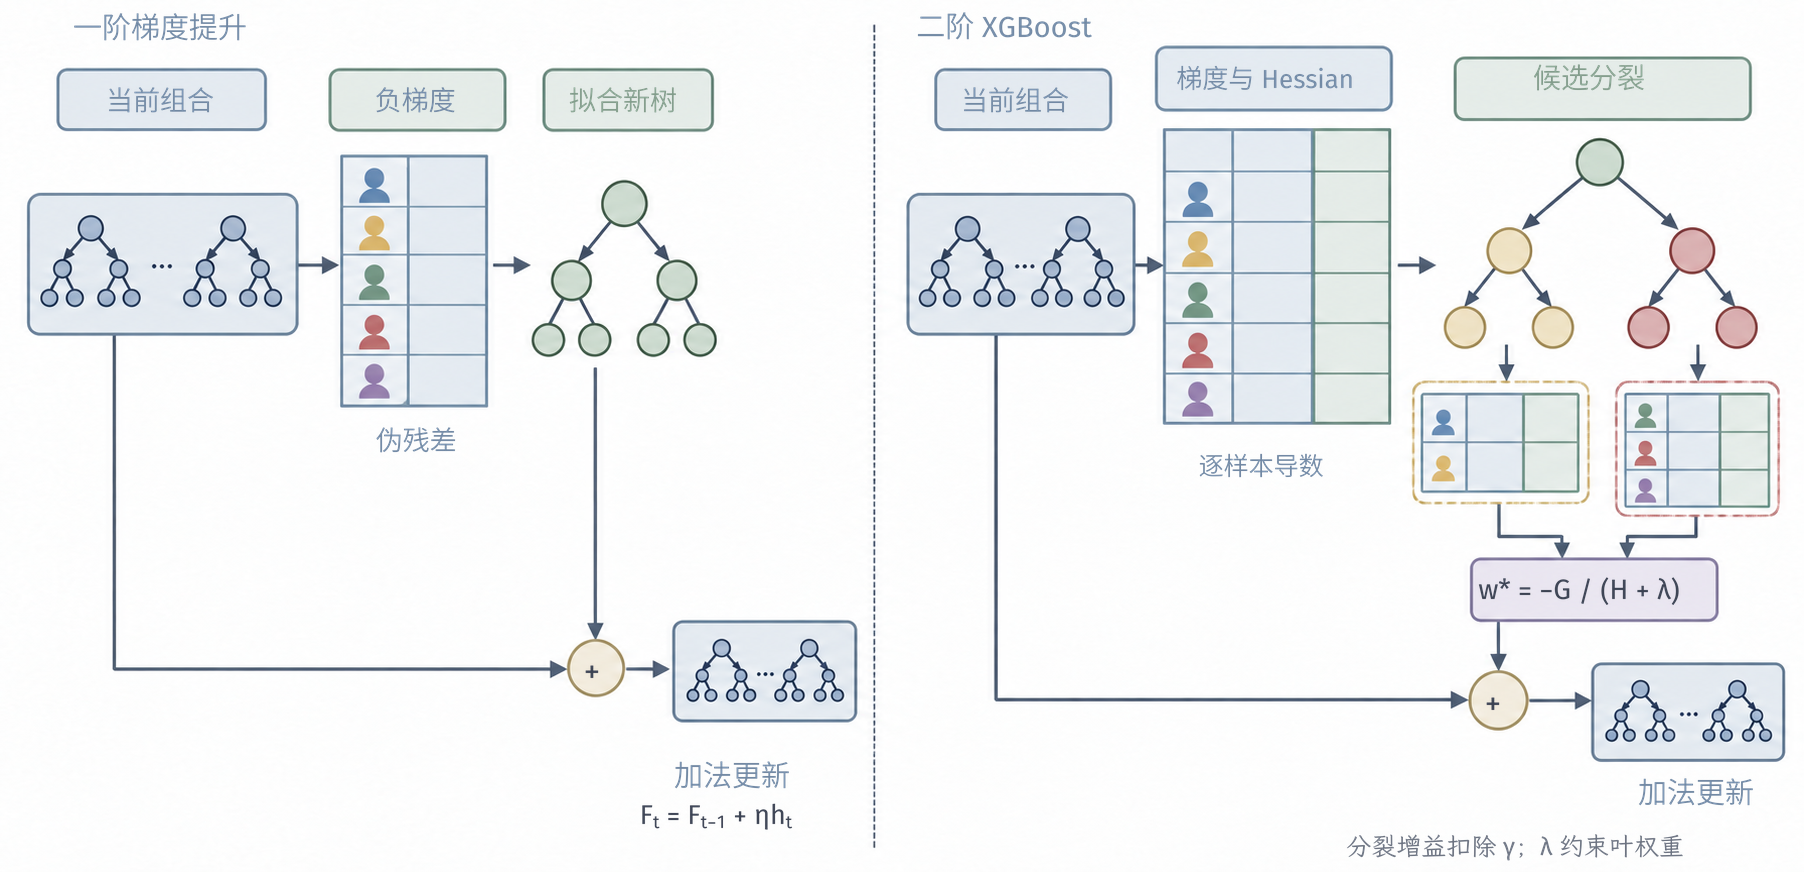
\includegraphics[width=152.739mm]{figures/04-classic-models/00-shared/generated/ensemble-gradient-xgboost/figure.png}
  \caption{梯度提升与XGBoost中的本轮修正。左图中，损失对当前预测的负梯度形成伪残差，新成员拟合该信号后更新组合；右图中，XGBoost按候选分裂聚合一阶导与二阶导，再由同一组叶统计计算叶权重和分裂增益。图中单叶权重$w^\ast$对应正文的$v_j^\star$，$G$与$H$分别表示叶内一阶导和二阶导之和。复杂度项$\gamma T+\lambda\lVert\bm{w}\rVert_2^2/2$中的$T$为叶数，$\bm{w}$汇集各叶输出；$\lambda$限制叶权重，$\gamma$惩罚新增叶。该图展示当前候选树的局部评分。}
  \label{fig:ensemble-gradient-xgboost}
\end{figure*}

\subsubsection{优化计算能力}

\paragraph{减少分裂搜索与数据访问}

精确分裂搜索遍历排序后的候选特征值；近似搜索则先用带权分位数草图构造候选切分，再汇总梯度统计。稀疏感知搜索为缺失值学习默认方向，列采样减少每轮需要检查的特征。块式存储、缓存感知访问、并行统计和外存计算改变的是实现代价，不改变式\eqref{eq:ensemble-xgboost-objective}所定义的学习对象。这些设计在特定硬件和数据规模上的时间收益可通过完整训练测量确认。

\Needspace{10\baselineskip}
\subsection{LightGBM}
\label{sec:ensemble-lightgbm}

\subsubsection{模型结构}

LightGBM仍以回归树的加法组合作为预测函数，树叶输出修正量，最终按任务所需把累计得分转换为预测。它主要改变如何在大规模数据上训练这些树。候选分裂的搜索可能成为提升树训练的主要成本。假设当前节点的一个连续特征有十万个不同取值，精确搜索就可能需要比较近十万个切分位置；每棵新树都会再次进行类似计算。\term{LightGBM}以直方图训练为基础，先把连续特征映射到有限个桶，再按桶累计梯度和曲率。如果使用256个桶，分裂评分就只在相邻桶之间比较，原来同桶内的差别被暂时忽略。

\subsubsection{参数学习}

构造直方图仍要访问节点样本，但候选搜索只需扫描桶。已知父节点和一个子节点的直方图时，还可以用差分得到另一个子节点的统计量。分桶减少存储和候选数，也引入离散化误差；桶数决定这种取舍。

树的生长顺序进一步改变计算分配。按层生长同时扩展某一深度上的叶，按叶生长则每次选择当前增益最大的叶继续分裂。在相同叶数下，后者把容量集中到训练目标下降较大的局部区域，可能形成深度不均衡的树。叶数、最小叶样本量和深度共同限制这种局部扩展，训练收益再由验证或测试检查其样本外效果。

\subsubsection{优化计算能力}

\paragraph{减少样本统计量}

基本直方图训练仍需统计大量样本和特征。LightGBM论文进一步提出两种针对这些成本的近似。\term{单边梯度采样}（gradient-based one-side sampling, GOSS）保留绝对梯度较大的样本，从绝对梯度较小的样本中随机抽取一部分，并在分裂统计中重新加权后者。例如，在小梯度组内等概率抽取一半样本，就把被抽中者对梯度和的贡献乘二，以补偿未采样部分。一般地，样本以概率$p>0$被保留时，其贡献乘以$1/p$；给定本轮梯度和候选分区，这种逆包含概率加权可无偏估计相应的梯度和，平方、比值及择优得到的增益则是非线性量，其偏差需另行分析。

\paragraph{减少有效特征数}

\term{互斥特征捆绑}（exclusive feature bundling, EFB）把很少同时非零的稀疏特征编码到较少的组合特征中，近似减少有效特征数。GOSS、EFB和直方图分别减少样本统计、特征表示和阈值候选，可按各自近似对象评价误差与计算节省\scite{ke2017lightgbm}。

图\ref{fig:ensemble-lightgbm-approximations}按近似对象并列这三种机制。直方图压缩候选阈值，GOSS压缩参与分裂统计的样本，EFB压缩稀疏特征表示；这三个对象分别对应数据访问、有效特征数与候选扫描的成本。

\begin{figure*}[t]
  \centering
  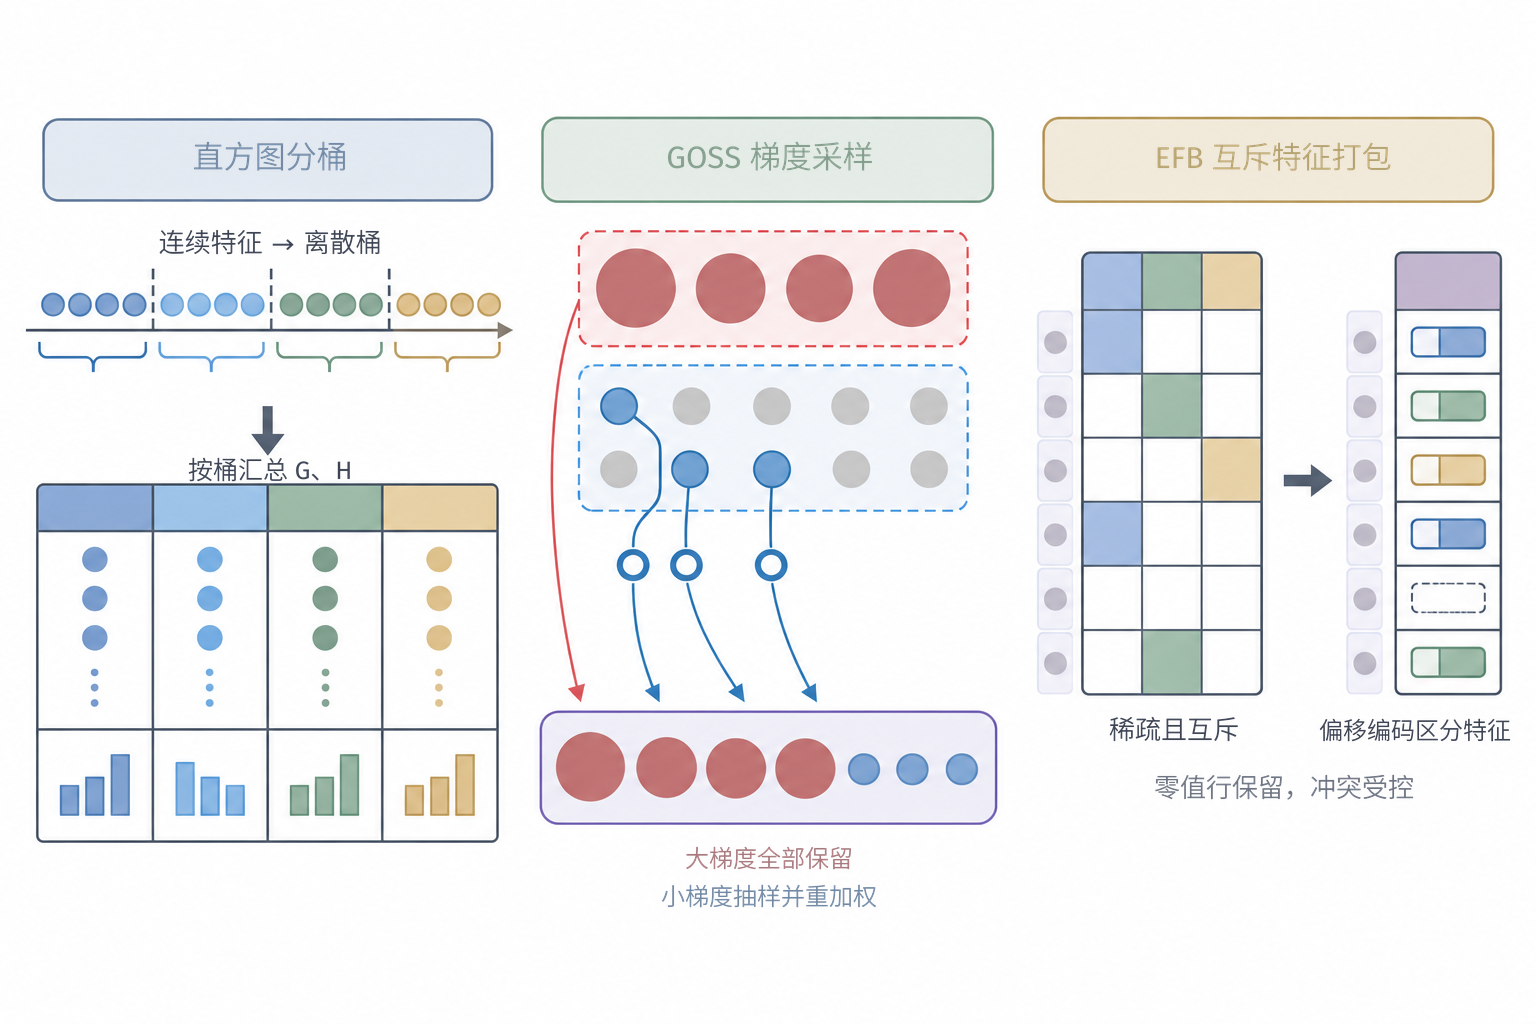
\includegraphics[width=130.048mm]{figures/04-classic-models/00-shared/generated/ensemble-lightgbm-approximations/figure.png}
  \caption{LightGBM中三种作用位置不同的计算近似。直方图把连续取值映射到有限桶，GOSS保留$|g_i|$较大的样本，并抽取、重加权部分$|g_i|$较小的样本，EFB把很少同时非零的特征编码为较少的捆绑特征。图中点数、桶数与非零位置均为机制示意。}
  \label{fig:ensemble-lightgbm-approximations}
\end{figure*}

这些机制的效果依赖梯度分布、特征稀疏性、桶数、冲突处理和硬件实现。比较速度和任务损失时，需要记录数据规模、硬件、桶数与采样设置，并固定搜索预算及早停规则。论文实验的结论据此限定于相应条件。GOSS对固定候选分区的梯度统计可以无偏，并不意味着据此选出的模型已经获得较低的期望风险。

\subsection{CatBoost}
\label{sec:ensemble-catboost}

\subsubsection{模型结构}

类别特征又带来不同的困难。例如商户标识可能有很多取值，全部展开为独热变量会增加特征规模，直接编成整数又会引入原本不存在的次序。用同类别记录的响应均值编码，可以把类别转成一个数，却容易把标签带回输入：某个商户若只有一条记录，包含该记录自身的响应均值恰好就是$y_i$，训练模型于是能直接读到待预测值。新记录的标签还未知，部署时无法提供同样信息。这种把待预测响应用于训练输入的构造称为\term{目标泄漏}（target leakage）。

\term{CatBoost}仍通过逐轮相加的树模型形成预测，并为类别特征安排避免当前标签泄漏的编码过程。它常使用\term{对称树}（symmetric tree），即同一深度的所有节点采用相同分裂条件。深度为$d_{\mathrm{tree}}$的完整对称树至多有$2^{d_{\mathrm{tree}}}$片叶，路径可以编码为固定长度的二进制选择。这种结构便于批量预测，也限制了单棵树可表达的分区形状。

\subsubsection{参数学习}

CatBoost用随机排列建立\term{有序目标统计}（ordered target statistic）。设$c_i$为样本$i$的某个类别值，用$\pi(j)$表示样本$j$在随机排列中的位置；对当前样本只使用排列中位于它之前且类别相同的记录：
\begin{equation}
  z_i
  =
  \frac{
    \sum_{j:\,\pi(j)<\pi(i)}
    \mathbb{I}\{c_j=c_i\}y_j
    +ap
  }{
    \sum_{j:\,\pi(j)<\pi(i)}
    \mathbb{I}\{c_j=c_i\}
    +a
  }.
  \label{eq:ensemble-catboost-ordered-statistic}
\end{equation}
其中$p$是先验统计量，$a>0$控制平滑。前缀统计排除了样本自身的标签，部署时可从已观测的训练记录形成同类别统计。低频类别仍会产生较大估计波动，平滑、多个排列和类别组合需要共同考虑。

图\ref{fig:ensemble-catboost-ordered-statistics}固定当前样本的排列位置，检查哪些标签进入编码。计算当前类别$A$样本的编码时，只允许排列前缀中同为类别$A$的标签进入统计量；其他类别、当前标签和排列后缀都不参与这次编码。

\begin{figure*}[htbp]
  \centering
  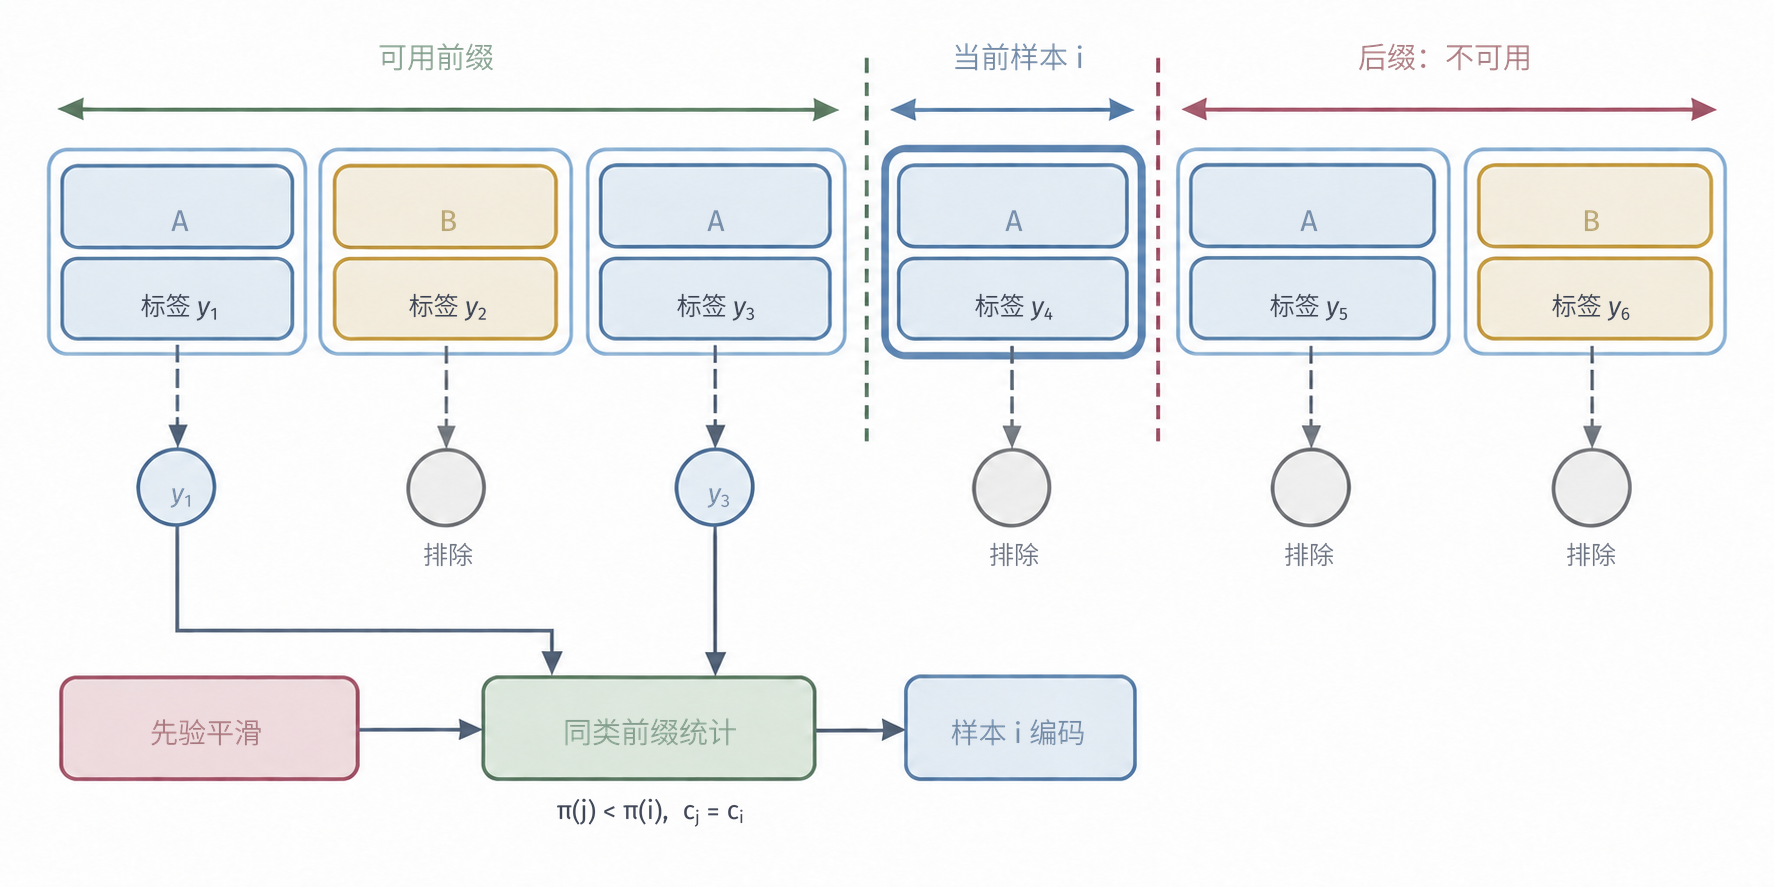
\includegraphics[width=150.199mm]{figures/04-classic-models/00-shared/generated/ensemble-catboost-ordered-statistics/figure.png}
  \caption{CatBoost有序目标统计的前缀约束。这里$\pi(j)$表示样本$j$在随机排列中的位置；计算当前样本$i$的编码时，只有满足$\pi(j)<\pi(i)$且$c_j=c_i$的标签通过实线汇入统计量。其他类别、当前标签和后续记录均不连接到统计量，表示它们在本次编码中被隔离。样本索引与类别符号仅用于说明机制。}
  \label{fig:ensemble-catboost-ordered-statistics}
\end{figure*}

有序提升把相同的前缀思想用于梯度估计。计算当前样本的预测与梯度时，采用由其前缀记录拟合的相应模型，使该样本的标签与当前预测拟合分离，以减少这一重复使用带来的预测偏移。实际算法通过多个排列和前缀模型实现这一约束，训练状态与计算量也比普通单序列提升更复杂\scite{prokhorenkova2018catboost}。

\subsection{模型对比与总结}
\label{sec:ensemble-boosting-comparison}

这些方法首先区别在“下一轮学什么”。AdaBoost由指数损失导出样本重加权，使错分记录影响后续分类器；GBM从一般损失导出负梯度，让成员拟合连续修正量，因而可以通过改变损失支持回归、概率分类和分位数预测。GBDT是以回归树拟合修正量的GBM实例。随机梯度提升和DART在这条序贯链上引入不同扰动，分别改变本轮样本与本轮所见的已有组合。

树提升还需要决定“怎样把修正量分配给叶区域”。XGBoost把损失曲率、叶权重惩罚和叶数代价合入局部评分，使候选分裂和叶输出可以用同一组统计计算。LightGBM进一步针对样本多、特征多、阈值候选多的计算成本，采用直方图、GOSS和EFB压缩相应对象，并按叶生长分配树容量。这些计算设计可以与损失及正则选择配合，代价是分桶、采样和特征捆绑带来的近似，不能仅凭方法名称判断速度或预测优劣。

CatBoost关注类别特征和标签重复使用的问题。它用排列前缀构造目标统计，并用前缀模型形成有序梯度，减少当前标签同时参与编码或预测拟合所造成的偏移；对称树则约束分区结构并便于批量预测。它与XGBoost、LightGBM共享树提升的外层结构，主要设计重点分别落在不同位置。表\ref{tab:ensemble-boosting-comparison}据此比较修正信号、局部目标、分裂计算与类别信息的使用方式。

\begin{table*}[htbp]
  \centering
  \small
  \begin{tabularx}{\linewidth}{@{}>{\raggedright\arraybackslash}p{19mm}*{6}{>{\raggedright\arraybackslash}X}@{}}
    \toprule
    方法 & 本轮修正信号 & 典型成员 & 目标近似 & 树生长或分裂 & 类别特征重点 & 主要约束 \\
    \midrule
    AdaBoost & 加权错分 & 树桩或浅分类树 & 指数损失下的解析更新 & 由成员算法决定 & 需另行编码 & 对持续错分记录敏感 \\
    GBM／GBDT & 负梯度伪残差 & 回归树 & 一阶函数方向与叶内优化 & 通常贪心树生长 & 需随实现处理 & 学习率、轮数与树复杂度耦合 \\
    XGBoost & 一阶导与二阶导 & 正则化回归树 & 二阶局部目标 & 精确或分位数候选；稀疏默认方向 & 依实现与版本而定 & 轮次串行，近似与系统配置影响成本 \\
    LightGBM & 桶级梯度统计 & 直方图回归树 & 通常使用二阶统计 & 按叶生长；直方图候选 & 支持类别分组，机制依实现 & 分桶、GOSS与EFB引入近似条件 \\
    CatBoost & 有序统计与有序梯度 & 对称树 & 梯度或二阶统计 & 同层共享分裂条件 & 有序目标统计与组合 & 多排列和前缀状态增加训练成本 \\
    \bottomrule
  \end{tabularx}
  \caption{Boosting代表方法的机制比较。GBM是一般框架，GBDT指使用回归树成员的实例；XGBoost、LightGBM和CatBoost是树提升的具体模型与系统，均属于Boosting框架的具体构造。}
  \label{tab:ensemble-boosting-comparison}
\end{table*}

提升方法都围绕当前组合继续训练，学习率、轮数和单树容量因而需要联合选择。若已有成员来自不同模型族，希望根据它们的样本外表现学习组合方式，就转向Stacking。

\section{基于Stacking的集成}
\label{sec:ensemble-stacking}

Bagging按固定规则聚合受到扰动的成员，Boosting则在逐轮训练中确定新成员的贡献。实际还可能已经有几种独立开发的模型。例如，同一房价任务中的线性模型概括整体趋势，近邻模型利用相似房屋的局部记录，森林表达特征交互。只挑一个模型会舍弃其他预测；一律等权平均又预先认定它们应当贡献相同。我们希望由数据学习怎样组合这些已有预测。

\term{Stacking}（stacked generalization，堆叠）把成员预测作为新特征，再训练一个组合模型。基学习器产生一级预测，\term{元学习器}（meta-learner）根据这些预测估计最终输出。元学习器可以学习线性权重，也可以在受控的函数类中学习非线性组合；是否能得到收益，取决于成员的样本外预测是否提供了互补信息\scite{wolpert1992stacked,breiman1996stacked}。

\subsection{Stacking}
\label{sec:ensemble-stacking-model}

\subsubsection{模型结构}

Stacking由基成员和元学习器两层组成，预测函数为
\[
 H(\bm x)=g_{\bm\theta}\!\left(h_1(\bm x),\ldots,h_M(\bm x)\right).
\]
其中$h_m$负责提取各自的预测信息，$g_{\bm\theta}$学习组合关系。基成员先对同一输入产生预测，元学习器把这些预测作为特征，输出最终结果。成员可以属于不同模型族；组合能够表达哪些关系，取决于元学习器允许的函数形式。

\subsubsection{参数学习}

\paragraph{生成折外训练特征}

设第$m$个成员模型为$h_m$。最直接的想法是：先在完整训练集上训练好每个成员，再把它们对训练样本的预测$h_m(\bm{x}_i)$当作元特征，喂给元学习器去学组合权重。这样做有一个隐蔽而致命的陷阱。设想成员中有一个“死记硬背”的模型，比如$1$近邻：它对每条训练记录的预测就是这条记录自己的标签，训练集上的正确率是$100\%$。元学习器看到这样的元特征，自然会认定“这个成员永远对，全听它的”，于是把几乎全部权重给它。可一到新样本，$1$近邻的表现可能远不如其他成员，元学习器学到的组合也就完全不可靠。问题的根源是：成员在训练记录上的预测已经“偷看过”这些记录的答案，而部署时成员面对的是没见过答案的新输入，两种预测的可信度完全不同；元学习器必须在“成员没见过答案”的条件下学习，才能学到对新样本有效的组合。

怎样让每条训练记录都得到一份“成员没见过它答案”的预测？交叉验证给出了答案，Stacking据此生成\term{折外预测}（out-of-fold prediction, OOF prediction）。思路是“轮流留出”：把训练样本划分为$K$个互不相交的折$V_1,\ldots,V_K$，每次留出一折、用其余折训练成员，再让它去预测被留出的那一折；轮完$K$次，每条记录都恰好被一个“没用它训练过”的成员预测过一次。具体地，对每个成员类型$m$和每个折$k$，只用$D_n\setminus V_k$训练临时模型$h_m^{(-k)}$，再预测$V_k$中的样本。若样本$i$属于$V_{k(i)}$，元特征定义为
\begin{equation}
  z_{i,m}
  =
  h_m^{(-k(i))}(\bm{x}_i).
  \label{eq:ensemble-oof-feature}
\end{equation}
把所有成员的折外预测拼成$\bm{z}_i=(z_{i,1},\ldots,z_{i,M})^{\top}$，再由元学习算法$\mathcal{G}$训练
\[
  g=\mathcal{G}\!\left(\{(\bm{z}_i,y_i)\}_{i=1}^{n}\right).
\]
对每个样本，临时成员的拟合数据排除了它所在的折，其标签只在后续元学习器训练中使用。图\ref{fig:ensemble-stacking-oof}展示了折外矩阵的形成过程。

\begin{figure*}[htbp]
  \centering
  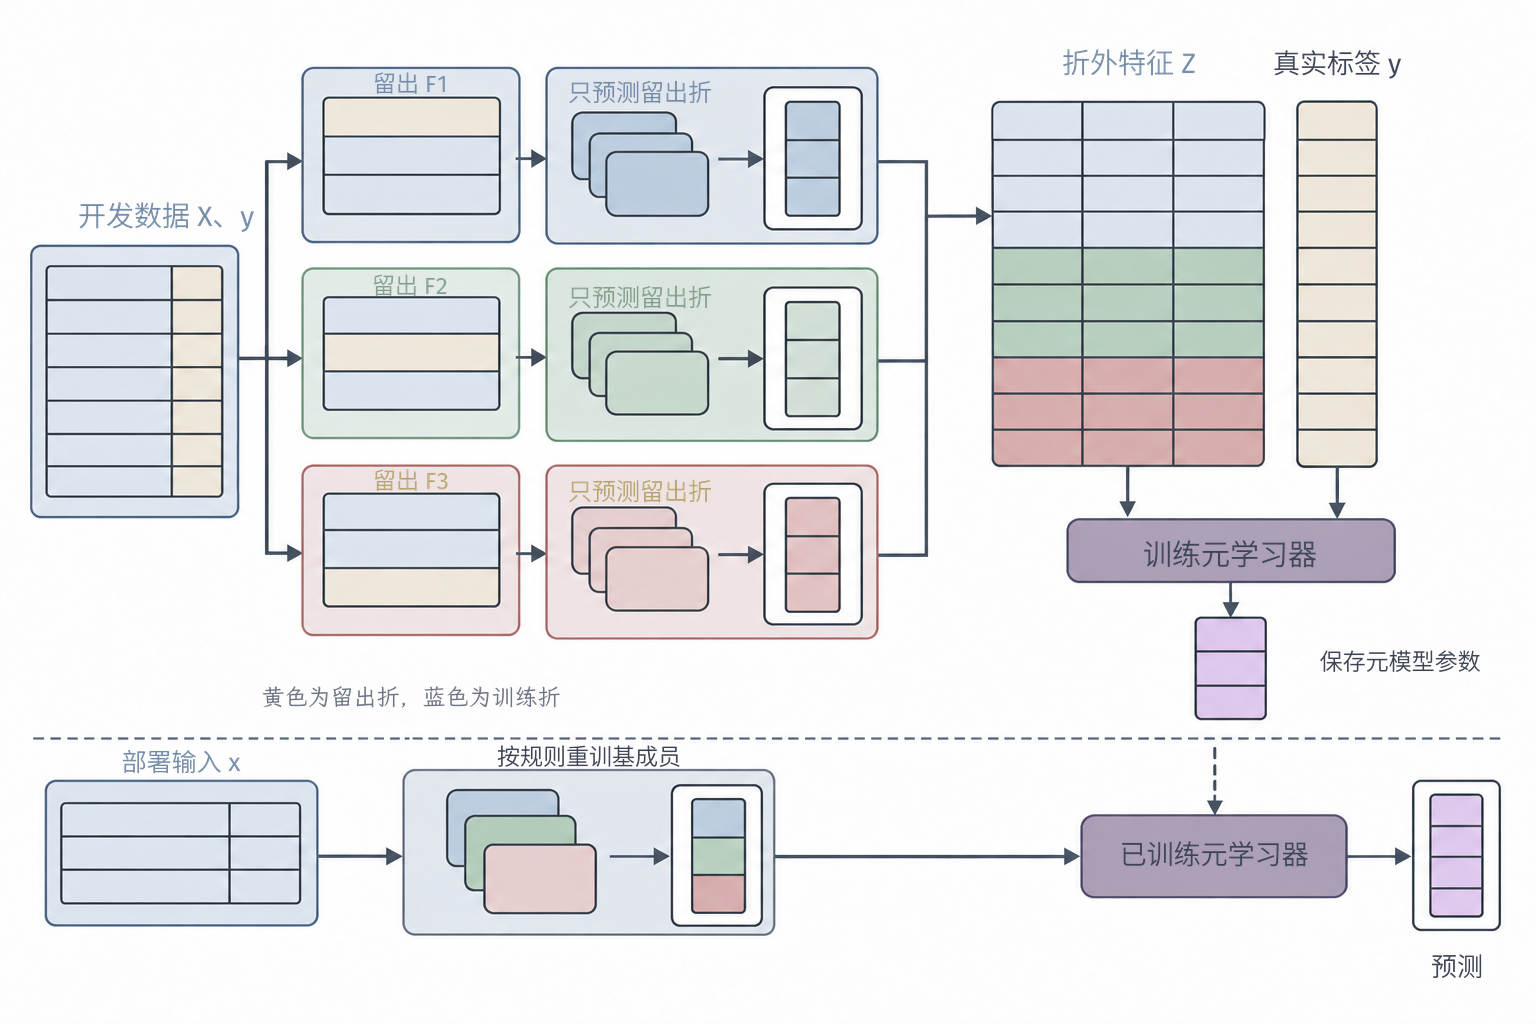
\includegraphics[width=130.048mm]{figures/04-classic-models/00-shared/generated/ensemble-stacking-oof/figure.png}
  \caption{三折Stacking的折外特征构造。每一折轮流作为留出折，临时成员只在其余两折训练，并为留出折产生预测；拼接三次预测得到完整折外矩阵$\bm{Z}$，元学习器以$\bm{Z}$为输入并使用对应标签拟合。部署阶段的基成员还需按预先规定的方式重训或保留。}
  \label{fig:ensemble-stacking-oof}
\end{figure*}

分类成员若输出$C$维概率向量，一个成员通常贡献$C$列元特征；二分类时也可以只保留一个类别概率。类别硬判断省去了得分中的排序或置信信息，不同成员的得分还可能采用不同尺度。元训练与部署使用一致的输出形式，正则化再控制尺度及相关预测对组合的影响。

\paragraph{确定部署成员}

折外矩阵用于训练元学习器，但部署时还需要能预测新输入的基成员。一种做法是在完整训练集上重新拟合每类基学习器$\widehat{h}_m$，预测
\[
  \widehat{y}
  =
  g\!\left(
    \widehat{h}_1(\bm{x}),\ldots,\widehat{h}_M(\bm{x})
  \right).
\]
全量重训利用全部开发数据，但训练规模增加可能改变预测分布，元学习器训练时只看过较小训练集产生的输出。也可保留各折成员，先平均它们对新输入的预测，再送入元学习器；这样沿用折内模型，同时增加了存储与推理次数。两方案的输入分布差异仍由完整验证检验。

部署方案确定后，需要评价基成员与元学习器共同形成的预测流程。基学习器的特征处理、类别编码和超参数搜索必须在相应训练折内完成。若先用全部数据选择特征或编码，再只把模型拟合放进交叉验证，信息仍可能从留出折进入元特征。

\subsubsection{多层组合与输入相关权重}

\paragraph{支持多层组合关系}
\label{sec:ensemble-stacking-multilevel}

若一层组合仍不足以描述成员间关系，可以把中间层输出继续送入下一层。令$\bm a_0(\bm x)=(h_1(\bm x),\ldots,h_M(\bm x))^{\top}$，多层结构写为
\[
 \bm a_\ell(\bm x)=g_{\ell,\bm\theta_\ell}(\bm a_{\ell-1}(\bm x)),
 \quad \ell=1,\ldots,L,
 \qquad H(\bm x)=\bm a_L(\bm x),
\]
其中最后一层维数与所需输出一致。也可把原始特征或较早层输出拼接到某层输入，但须明确拼接对象。训练第$\ell$层时，对每个留出折，都要在其余数据上重新拟合完整下层流程，再为该折产生$\bm a_{\ell-1}$。只让底层成员留出当前记录，而让中间组合层使用其标签，仍会泄漏。逐层增加表达能力的代价是重复拟合、更多参数与部署计算，需要用完整外层验证判断是否值得。

\paragraph{支持输入相关组合}
\label{sec:ensemble-stacking-input-dependent}

固定线性权重让所有输入使用同一组成员贡献。如果线性模型在稀疏区域更稳定、近邻模型在稠密区域更准确，可以让权重随输入改变。一种具体结构是用门控函数$b_m(\bm x;\bm\theta)$产生非负归一化权重：
\[
 w_m(\bm x;\bm\theta)
 =\frac{e^{b_m(\bm x;\bm\theta)}}{\sum_{j=1}^M e^{b_j(\bm x;\bm\theta)}},
 \qquad
 H(\bm x)=\sum_{m=1}^M w_m(\bm x;\bm\theta)h_m(\bm x).
\]
基成员固定后，用折外预测$z_{i,m}$估计门控参数：
\[
 \widehat{\bm\theta}\in\argmin_{\bm\theta}
 \sum_i\ell\!\left(y_i,\sum_m w_m(\bm x_i;\bm\theta)z_{i,m}\right)
 +\lambda\Omega(\bm\theta).
\]
门控输入也须按训练折预处理。部署时把折外预测替换为预定部署成员的输出；各类别概率可以用同一组权重逐类组合。这种加权仍计算全部参与成员，第\ref{sec:ensemble-dynamic-selection}节的动态选择则可进一步只调用一个成员或某个子集。

\subsection{Blending}
\label{sec:ensemble-blending}

\subsubsection{模型结构}

折外构造让每条训练记录都获得一份未使用自身标签的成员预测，却要为每种成员重复拟合多个折内模型。成员训练昂贵时，这个成本可能难以承担。\term{Blending}改用一次留出来构造元特征：把开发数据分为基训练集$D_{\mathrm{base}}$和组合训练集$D_{\mathrm{blend}}$，基成员只在前者拟合，再预测后者，元学习器用这些预测与对应标签训练。每种成员只需一次用于元特征的拟合，代价是两层不再都利用全部开发样本。

\subsubsection{参数学习}

训练数据由两层分用：基成员在$D_{\mathrm{base}}$拟合，元学习器只使用$D_{\mathrm{blend}}$的预测与标签。在开发数据总量固定时，组合训练集$D_{\mathrm{blend}}$占比较小，元学习器用于估计组合关系的记录较少，估计可能不稳定；$D_{\mathrm{blend}}$占比增大，留给基训练集$D_{\mathrm{base}}$的记录随之减少，基成员训练信息也会减少。多次随机划分并平均可以减小单次划分的偶然性，但它重新引入多次训练，已经不再具有单次Blending的全部成本优势。

部署时若把$D_{\mathrm{blend}}$加入基成员重新训练，基预测分布可能相对元学习器训练时发生变化；若不加入，则没有充分利用已有标签。重训方式因此属于模型配置，需要先确定，再用未参与选择的数据评价实际组合。

\Needspace{10\baselineskip}
\subsection{受约束线性Stacking}
\label{sec:ensemble-constrained-linear-stacking}

\subsubsection{模型结构}

成员预测往往高度相关。例如两棵森林只在少量输入上稍有差别，元学习器就可能用很大的正权重与负权重相互抵消，拟合这些细小差异；成员输出稍有变化，组合也会随之放大变化。若希望用较少参数组合，并限制这种抵消，可以把元学习器限制为$b+\bm w^{\top}\bm z$，其中$b$是截距，$\bm w$是成员权重，$\bm z$汇集成员预测。在截距为零且权重非负时，再把权重和限制为一，组合预测就落在成员预测的范围内。

\subsubsection{参数学习}

在回归折外矩阵$\bm{Z}\in\mathbb{R}^{n\times M}$上，可以通过带惩罚的经验目标估计截距与权重：
\begin{equation}
  (\widehat{b},\widehat{\bm{w}})
  \in
  \argmin_{b,\bm{w}}
  \frac{1}{n}
  \sum_{i=1}^{n}
  \ell\!\left(
    y_i,
    b+\bm{w}^{\top}\bm{z}_i
  \right)
  +\lambda\lVert\bm{w}\rVert_2^2.
  \label{eq:ensemble-linear-stacking}
\end{equation}
权重约束控制组合允许的尺度和方向。在$b=0$时，仅要求$w_m\geq0$得到非负线性组合，仍可能放大预测；仅要求$\sum_mw_m=1$得到仿射组合，仍可因负权重而外推。只有同时满足$b=0$、$w_m\geq0$和$\sum_mw_m=1$，才是成员预测的凸组合，输出必定位于成员预测的凸包内。非负约束排除了成员之间的正负抵消，归一化进一步限制整体尺度；有效校正若需要负权重或截距，约束会缩小候选类并增加逼近误差。

权重大小同时受输出尺度、成员相关性和损失函数影响。两个成员预测近乎相同，线性模型可以在它们之间任意分配相近作用；一个成员输出的数值范围更大，也会改变未标准化正则项下的权重。估计权重反映给定尺度、相关性与损失下的联合拟合，而非成员独立贡献。对同一类别集合上的概率向量，使用同一组满足上述凸组合条件的权重逐类组合，结果保持概率单纯形约束，样本外校准再检查概率与实际频率的对应。

\Needspace{10\baselineskip}
\subsection{Super Learner}
\label{sec:ensemble-super-learner}

\subsubsection{模型结构}

不同学习器各有合适的数据条件，事先往往难以指定最佳成员及权重。\term{Super Learner}把候选模型库、折外预测和损失最小化组织成完整程序：用同一套折外数据比较候选，再选择单个成员或学习受约束组合。回归中常用的组合结构为$H(\bm x)=\sum_m w_m h_m(\bm x)$，其中$w_m\geq0$且$\sum_mw_m=1$\scite{vanderlaan2007superlearner}。

\subsubsection{参数学习}

先按式\eqref{eq:ensemble-oof-feature}生成候选库的折外矩阵$\bm Z$。离散版本选择折外平均损失最小的一列；连续组合版本则求解
\[
 \widehat{\bm w}\in\argmin_{\bm w\in\Delta_M}
  \frac1n\sum_{i=1}^n\ell\!\left(y_i,\sum_{m=1}^M w_m z_{i,m}\right),
 \qquad
 \Delta_M=\{\bm w:w_m\geq0,\ \sum_mw_m=1\}.
\]
例如平方损失给出带单纯形约束的最小二乘问题。随后在全部开发数据上重训各基成员，保留已学权重用于组合。候选库也可以预先包含不同模型族和超参数设置，但每列的折外预测必须遵守相应训练范围。

这里的折外损失参与了权重选择，不能再充当整个Super Learner未经选择的最终测试结果。若要比较不同候选库、组合约束或完整Stacking程序，应在外层验证中重新完成内层训练与权重选择。Super Learner与受约束Stacking因此可以共享同一预测结构；前者强调候选库及交叉验证选择程序，后者强调组合层的形式。

\subsection{模型对比与总结}
\label{sec:ensemble-stacking-comparison}

这些方法改变的是组合训练的不同环节。Stacking与Blending分别采用折外预测与一次留出预测；受约束线性组合限制元学习器，多层结构增加组合深度，门控结构使权重依赖输入。Super Learner进一步把候选库和交叉验证损失规定为完整选择程序。表\ref{tab:ensemble-stacking-comparison}据此比较数据安排、组合方式及成本。

\begin{table*}[htbp]
  \centering
  \small
  \begin{tabularx}{\linewidth}{@{}>{\raggedright\arraybackslash}p{25mm}*{5}{>{\raggedright\arraybackslash}X}@{}}
    \toprule
    方法 & 元特征来源 & 数据利用 & 组合规则 & 主要成本 & 主要风险 \\
    \midrule
    Stacking & $K$折折外预测 & 每个样本都产生元特征 & 可线性或非线性 & 每类成员需多次折内拟合 & 折外流程不完整造成泄漏 \\
    Blending & 固定留出集预测 & 元学习器只用留出集 & 可线性或非线性 & 基成员用于元特征时只拟合一次 & 划分敏感与重训分布变化 \\
    受约束线性Stacking & 通常为折外预测 & 与所用划分一致 & 非负、和为一或正则化线性组合 & 组合层较轻量 & 约束可能排除有效校正 \\
    Super Learner & 交叉验证预测与风险 & 由交叉验证方案决定 & 在预定库和组合类中选择 & 候选库越大，训练与选择成本越高 & 候选库遗漏合适模型，或选择过程泄漏 \\
    \bottomrule
  \end{tabularx}
  \caption{Stacking及其代表性变体。表中“数据利用”描述元学习器训练阶段；部署前是否用完整开发数据重训基成员，还需作为流程的一部分单独规定。}
  \label{tab:ensemble-stacking-comparison}
\end{table*}

部署前的全量重训还会改变成员产生预测时所用的训练规模。选择保留折内成员还是重训成员，需要与组合层一起评价，不能只比较各基成员的单独测试结果。比较上述方法时，应固定输出语义、预处理范围和训练预算，再判断新增组合是否改善完整流程的预测。

\section{成员选择与集成简化}
\label{sec:ensemble-selection-compression}

Bagging、Boosting和Stacking先回答怎样形成组合。部署时，多成员推理可能超出内存或延迟预算，一些成员也可能只在局部输入上有用。简化集成有三种不同目标：为所有输入固定一个较小成员子集，针对当前输入临时选择成员，或训练一个新的紧凑模型替代原集成。前两种方法保留部分原成员，第三种方法改变了部署模型。

图\ref{fig:ensemble-selection-compression}沿部署对象区分这三种目标。静态选择把成员池缩成一个固定子集，动态选择保留成员池并让路由依赖当前输入，紧凑化则把完整集成的行为转移到新模型。资源评价据此包括被部署模型以及选择或路由计算。

\begin{figure*}[htbp]
  \centering
  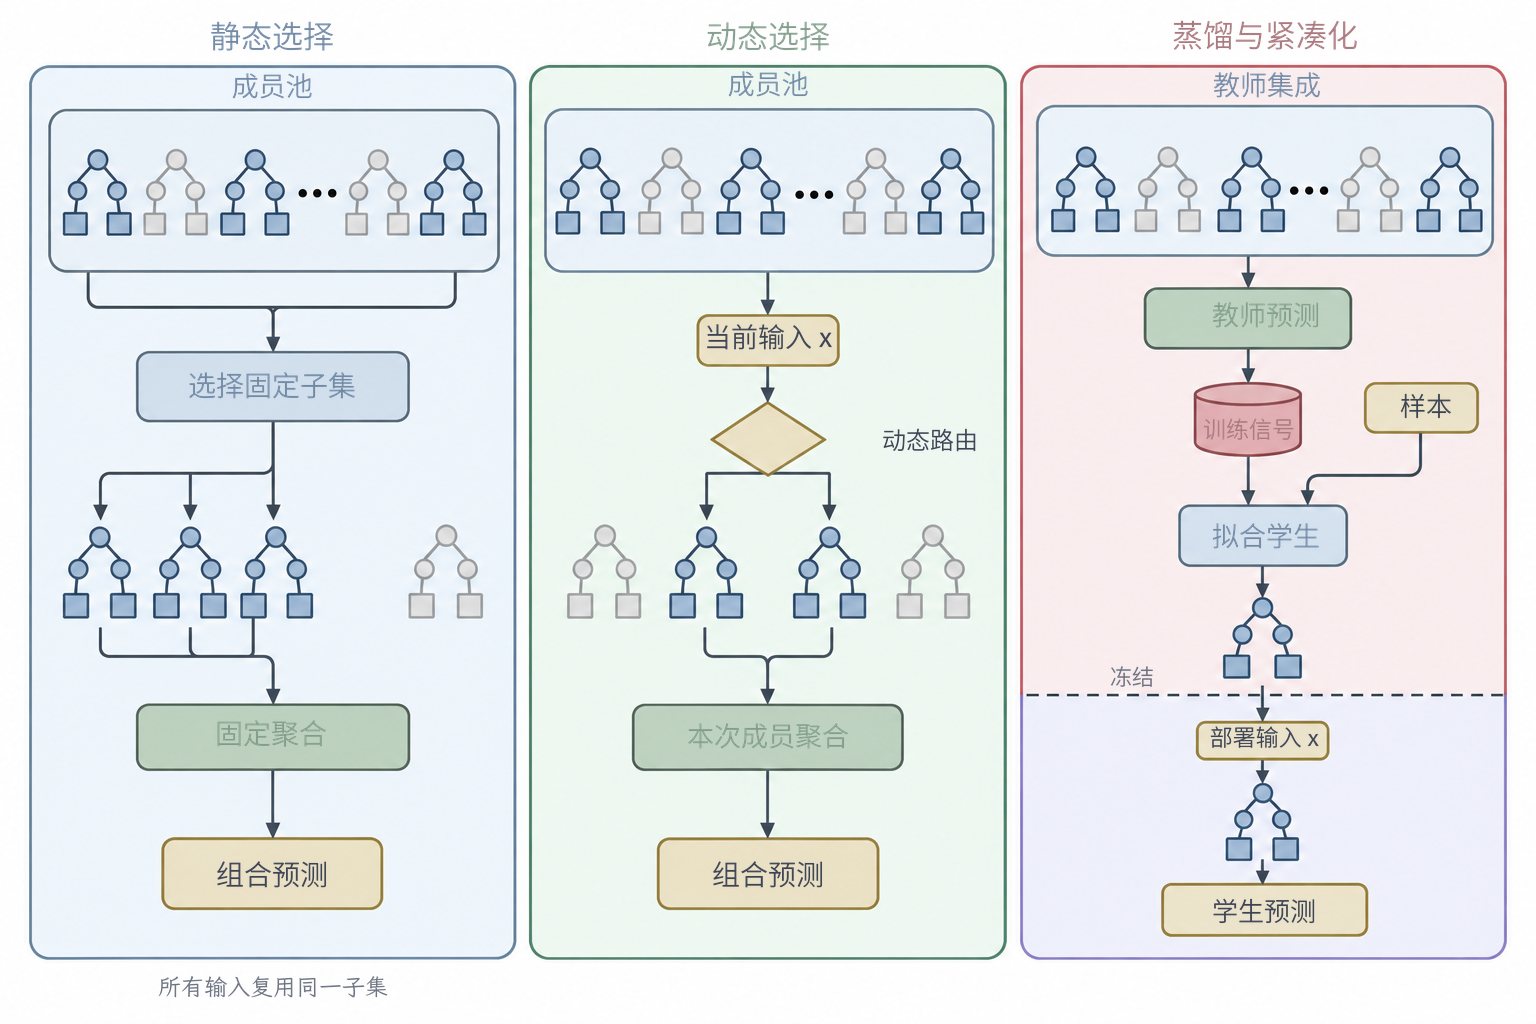
\includegraphics[width=130.048mm]{figures/04-classic-models/00-shared/generated/ensemble-selection-compression/figure.png}
  \caption{静态成员选择、动态成员选择与紧凑化改变的部署对象。静态选择为所有输入保留同一成员子集；动态选择根据输入改变运行成员或组合权重；紧凑化训练并部署新的学生模型。三种路径改变的计算对象不同，成本需沿各自完整路径测量。}
  \label{fig:ensemble-selection-compression}
\end{figure*}

\subsection{静态成员选择}
\label{sec:ensemble-static-selection}

\subsubsection{模型结构}

部署时若只能保留部分成员，我们需要选择在预算内预测效果合适的组合。单模型评分还不足以作出选择：几份预测近乎相同的强成员可能互相重复，加入一个单独误差稍大、但能纠正它们共同错误的成员，反而可能得到更好的组合。\term{静态成员选择}（static ensemble selection）从已经训练好的候选池$\{h_1,\ldots,h_M\}$中，选择一个对所有未来输入都相同的非空子集$S\subseteq\{1,\ldots,M\}$，评价对象是整个子集的组合预测。

\subsubsection{参数学习}

若$\mathcal{L}_{\mathrm{val}}(S)$表示该组合的平均验证损失，可以用损失与部署成本共同选择子集：
\begin{equation}
  \widehat{S}
  \in
  \argmin_{\varnothing\neq S\subseteq\{1,\ldots,M\}}
  \mathcal{L}_{\mathrm{val}}(S)
  +\lambda_1|S|
  +\lambda_2 C(S),
  \label{eq:ensemble-static-selection}
\end{equation}
其中$\lambda_1,\lambda_2\geq0$，$|S|$控制成员数，$C(S)$可以表示存储、单样本延迟或其他部署成本。成员池包含指数多个子集，实际可用排序、逐个加入或删除等方法近似搜索，并记录所得子集的验证损失与资源成本。

单成员排序忽略预测的重叠，可能同时保留许多相似模型。前向选择则评价候选加入当前组合后的损失变化，使选择依赖已有成员。允许重复选择某个成员时，重复次数还形成离散权重。基于模型库的贪心集成选择就是这种做法的代表：从一个初始组合出发，每轮加入使验证指标改善最大的候选，必要时使用多起点或装袋法减少搜索的不稳定性\scite{caruana2004ensemble}。

式\eqref{eq:ensemble-static-selection}的搜索对象为固定池中的成员子集，成员预测已经形成。若同时改变基学习算法、特征处理和超参数，搜索范围已经扩展为完整模型开发流程。候选池越大，验证集上偶然出现有利组合的机会也越多；最终测试需在该子集及其组合规则固定后进行。

\subsection{动态成员选择}
\label{sec:ensemble-dynamic-selection}

\subsubsection{模型结构}

静态方案让所有输入使用相同子集，却可能遗漏成员能力随输入改变的情况。假设一个文本分类器在体育报道附近的预测可靠，另一个在科技报道附近更可靠，用全体文档上的平均正确率排序，就可能忽略这种局部差别。我们可以在独立数据中寻找与当前输入邻近的记录，比较成员在这些记录上的表现，再决定调用谁。\term{动态分类器选择}（dynamic classifier selection, DCS）为每个输入选择一个成员；\term{动态集成选择}（dynamic ensemble selection, DES）选择一个成员子集或给出输入相关权重。

\subsubsection{参数学习}

一种基本构造是准备独立的能力估计数据。对查询输入$\bm{x}$，在该数据中寻找非空邻域$\mathcal{N}(\bm{x})$，再以成员$m$在邻域内的正确率估计
\begin{equation}
  \widehat{c}_m(\bm{x})
  =
  \frac{1}{|\mathcal{N}(\bm{x})|}
  \sum_{i\in\mathcal{N}(\bm{x})}
  \mathbb{I}\!\left\{h_m(\bm{x}_i)=y_i\right\}.
  \label{eq:ensemble-local-competence}
\end{equation}
DCS可以选择$\widehat{c}_m(\bm{x})$最大的成员，DES则保留超过阈值的成员或按能力加权。局部正确率只是能力估计的一种方式，还可以使用输出轮廓、分类间隔或由元模型学习的能力特征\scite{woods1997localaccuracy}。

局部选择依赖邻域和能力估计两部分。邻域依赖输入表示与距离，高维或分布稀疏时，附近样本未必提供稳定的局部证据；能力估计器也可能在有限数据上过拟合。成员训练数据、能力估计数据与最终测试数据需要分开，所有标准化和邻域参数都在相应开发流程内确定。

动态选择的延迟由路由和实际运行成员共同决定。若系统必须先运行全部成员才能构造输出轮廓，再选择其中几个聚合，选择之前已经支付全部成员计算；基于输入邻域的方法还增加了检索成本。在昂贵成员运行前完成路由，才可能直接省去被跳过成员的计算；局部检索、路由和输出质量需要一并测量。

\subsection{从集成模型到紧凑模型}
\label{sec:ensemble-compression}

\subsubsection{模型结构}

若原成员的最小可用子集仍超预算，可以另外训练一个新的\term{紧凑模型}（compact model），使其逼近完整集成的输入输出映射。早期模型压缩工作已经用大型集成的输出训练较小模型；知识蒸馏随后把这种教师到学生的传递扩展为常用训练形式\scite{bucilua2006compression,hinton2015distilling}。

\subsubsection{参数学习}

设完整集成为教师$H$，紧凑模型为学生$s_{\bm{\theta}}$。对回归，可以组合真实响应损失与教师拟合损失：
\begin{equation}
  \min_{\bm{\theta}}
  \sum_{i=1}^{n}
  \left[
    \alpha\ell\!\left(y_i,s_{\bm{\theta}}(\bm{x}_i)\right)
    +(1-\alpha)
    \ell\!\left(H(\bm{x}_i),s_{\bm{\theta}}(\bm{x}_i)\right)
  \right],
  \label{eq:ensemble-compression-objective}
\end{equation}
其中$\alpha\in[0,1]$控制真实标签与教师输出的作用。分类时可以拟合教师的完整类别分布；温度缩放会使非最大类别之间的相对关系更容易进入训练信号，但温度、损失权重与部署概率仍须分别选择和校准。

学生训练输入可以来自原训练集、额外未标注样本或经过说明的合成样本。教师在所选输入上提供训练目标；覆盖不足的区域缺少这种监督，学生在这些区域仍可能偏离教师。学生容量过小会产生逼近误差，容量很大则可能无法达到预期资源节省。


\Needspace{18\baselineskip}
\section{本章小结}
\label{sec:ensemble-summary}

集成利用成员生成与组合规则改变预测误差。互补作用来自成员能够在部分输入上修正彼此的判断，共同遗漏的结构仍需改变表示或训练方式。Bagging通过样本、特征或分裂随机性构造可并行成员，再用平均或投票削弱一部分训练波动；Boosting让每轮成员依赖当前组合，沿选定损失逐步加入修正；Stacking使用折外预测训练元学习器，使组合规则本身也由数据决定。三类机制可以嵌套，但各自的数据依赖、计算路径和失效原因不同。

成员池形成后，还可以改变部署规模。静态成员选择为所有输入固定同一子集，动态成员选择针对当前输入估计局部能力，紧凑化则训练一个新模型逼近完整集成。选择保留原成员的部分计算，紧凑化则部署一个重新训练的预测器，因此其成本与误差来源需要分别评价。

三类方法的改进需要放在完整预测流程中判断。Bagging的成员可以并行训练，Boosting的轮次相互依赖，Stacking则同时承担基成员与组合层的计算；相同成员数并不意味着相同容量或成本。比较时应使用同一输出目标、数据划分和调参预算，同时检查任务损失、概率质量、模型大小以及包含预处理、全部成员和路由的端到端延迟。

图\ref{fig:ensemble-data-isolation}概括了不同留出预测的职责。袋外预测用于Bagging内部诊断，折外预测用于训练Stacking组合层，能力估计预测用于动态选择，验证预测用于确定配置；这些结果都可能影响模型开发。最终测试只评价成员、组合、校准和部署规则全部冻结后的流程。预处理、成员筛选和超参数搜索也必须留在相应训练范围内，不能只隔离最后一次模型拟合。后续神经网络模型部分将在这些原则上讨论初始化、样本顺序与训练过程产生的神经网络集成。

\begin{figure*}[htbp]
  \centering
  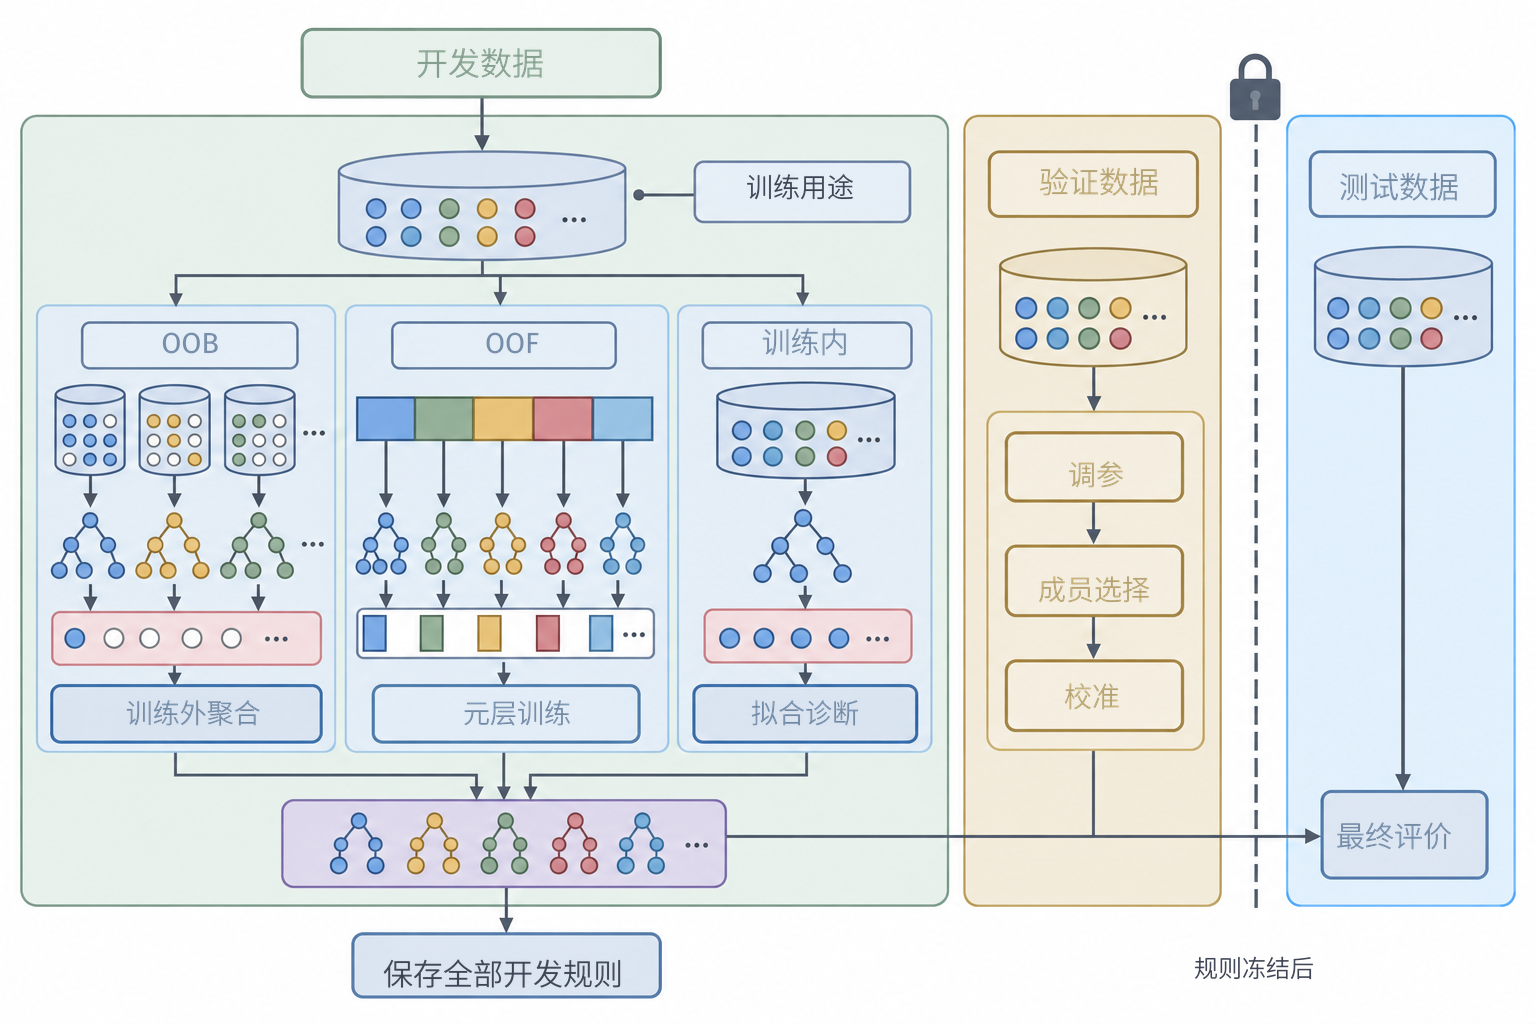
\includegraphics[width=130.048mm]{figures/04-classic-models/00-shared/generated/ensemble-data-isolation/figure.png}
  \caption{集成学习中的数据隔离与预测职责。开发阶段的预测及验证数据各有规定用途；测试阶段前的竖直分隔线表示训练、调参、筛选、校准和部署规则已经冻结。测试预测评价已经冻结的流程；图中不向开发步骤返回选择信号。}
  \label{fig:ensemble-data-isolation}
\end{figure*}

\paragraph{扩展阅读}
Hastie等的教材从加法建模解释提升方法；Breiman的Bagging与随机森林论文说明重采样及特征随机化的作用。可选同一预测任务，比较成员误差中可被组合削弱的部分，并记录获得这一收益所需的训练与部署成本\scite{hastie2009,breiman1996bagging,breiman2001randomforests}。
